% Nasza inżynierka
\documentclass[10pt,twoside,a4paper,hidelinks]{article}
\usepackage{fontspec}                 % żeby ustawić czcionkę na systemową (Arial)
\usepackage{geometry}                 % do marginesów
\usepackage{indentfirst}              % żeby pierwsze akapity też miały wcięcie
\usepackage{titlesec}                 % żeby formatować tytuły rozdziałów itd.
\usepackage{secdot}                   % aby dodać kropkę za numerkiem podrzodziałów i podpodrozdziałów
\usepackage{chngcntr}                 % umożliwia numerowanie obrazków itp. względem rozdziału
\usepackage{tocloft}                  % umożliwia ustawienia dotyczące spisu treści i innych spisów
\usepackage{tabu}                     % do tabel
\usepackage[table,dvipsnames]{xcolor} % do kolorowania tabel
\usepackage{tabularx}                 % do lepszych tabel
\usepackage[backend=bibtex]{biblatex} % do bibliografii
\usepackage{enumitem}                 % do modyfikacji listy (begin{itemize}, niepotrzebne odstępy przed i po)
\usepackage{floatrow}                 % aby umożliwić wymuszenie położenia figury
\usepackage{caption}                  % do zmiany podpisów tabel i obrazków
\usepackage{setspace}                 % również do zmiany podpisów (konkretniej interlinii w podpisach - wymagany przez caption)
\usepackage{longtable}
\usepackage{booktabs}
\usepackage{tabu}
\usepackage{changepage}
\usepackage{amsthm}
\usepackage{hyperref}
\usepackage[final]{pdfpages}
\usepackage{multirow}
\usepackage[titletoc,title]{appendix}
\usepackage{listings}
\usepackage{dirtree}
\usepackage{multicol}
\usepackage{subcaption}
\usepackage{amsmath,amssymb}
\DeclareMathOperator{\EX}{\mathbb{E}} % expected value

\newcommand\myicon[1]{{\color{#1}\rule{2ex}{2ex}}}
\newcommand{\myfolder}[2]{\myicon{#1}\ {#2}}
\newcommand\editnote[1]{\textcolor{red}{{\em [#1]}}} % See: https://tex.stackexchange.com/questions/9796/how-to-add-todo-notes

\definecolor{listinggray}{gray}{0.9}
\definecolor{lbcolor}{rgb}{0.9,0.9,0.9}
\lstset{
  backgroundcolor=\color{lbcolor},
  tabsize=4,
  language=Python,
  captionpos=b,
  tabsize=4,
  frame=lines,
  numbers=left,
  numberstyle=\tiny,
  numbersep=5pt,
  breaklines=true,
  showstringspaces=false,
  basicstyle=\linespread{0.94}\footnotesize\ttfamily,
% identifierstyle=\color{magenta},
  keywordstyle=\color[rgb]{0,0,1},
  commentstyle=\color{OliveGreen},
  stringstyle=\color{red}
  }


% Magia żeby dodatki miały ma początku "Dodatek X: ..."
\makeatletter
\renewcommand{\@redotocentry@pp}[1]{%
  \let\oldacl@pp=\addcontentsline
  \def\addcontentsline##1##2##3{%
    \def\@pptempa{##1}\def\@pptempb{toc}%
    \ifx\@pptempa\@pptempb
      \def\@pptempa{##2}\def\@pptempb{#1}%
      \ifx\@pptempa\@pptempb
        \oldacl@pp{##1}{##2}{\appendixname\space ##3}%
      \else
        \oldacl@pp{##1}{##2}{\chaptertitlename\space ##3}% added \chaptertitlename
      \fi
    \else
      \oldacl@pp{##1}{##2}{##3}%
    \fi}
}
\makeatother

% to jest jakas magia, aby odczytac szerokość longtable i ustawić tę wartość później jako LTcapwidth (parametr kontrolujący szerokość captiona w longtable)
% Creditsy i flaszkę proszę wysyłać do magika Heiko (http://compgroups.net/comp.text.tex/longtable-tablewidth/1922986)
\makeatletter
\newlength\LongtableWidth
\newcommand*{\org@longtable}{}
\let\org@longtable\longtable
\def\longtable{%
  \begingroup
    \advance\c@LT@tables\@ne
    \edef\x{LT@\romannumeral\c@LT@tables}%
    \global\LongtableWidth\z@
    \@ifundefined{\x}{%
      % longtable width not available
    }{%
      \def\LT@entry##1##2{%
        \global\advance\LongtableWidth##2\relax
      }%
      \@nameuse{\x}%
    }%
    % debug output
    \typeout{* \x: \the\LongtableWidth}%
  \endgroup
  \ifdim\LongtableWidth>\z@
    \setlength{\LTcapwidth}{\LongtableWidth}%
  \fi
  \org@longtable
}
\makeatother

% Rozpocznij od nowa numerowanie rysunków dla każdego rozdziału (section).
% Dodaje numer rozdziału do numeru rysunku: nr_rozdzial.nr_rysunku_w_ramach_rozdzialu
%
% Źródło: http://tex.stackexchange.com/questions/28333/continuous-v-per-chapter-section-numbering-of-figures-tables-and-other-docume
\counterwithin{figure}{section}

% to samo dla tabel
\counterwithin{table}{section}

% żeby nie było Rysunek tylko Rys
\renewcommand{\figurename}{Fig.}

% żeby nie było odstępów przed/po/w środku listy (itemize, ew. dodać też dla enumerate?)
\SetLabelAlign{parright}{\parbox[t]{\labelwidth}{\raggedleft#1}}
\setlist[itemize]{noitemsep,nolistsep,topsep=0pt}
\setlist[description]{noitemsep,nolistsep,topsep=0pt,style=multiline,align=parright}
    
% ustawiamy domyślny odstęp przed i po pływającymi elementami (tabele i obrazki) umieszczonymi w środku tekstu (flaga H) na 0
\setlength{\intextsep}{0mm}
\setlength{\textfloatsep}{0mm}

% ustawiamy domyślną czcionkę dla podpisów na small (9pt dla article 10pt) oraz interlinię na 1.0
\captionsetup{font={small,stretch=1.0}}

% własny separator do podpisów (to, co jest po 'Rys. X.Y' - kropka, nazwana wewnętrznie jako 'dot')
\DeclareCaptionLabelSeparator{dot}{. }
\DeclareFloatVCode{6ptskip}{\vspace{6pt}}
\DeclareFloatVCode{12ptskip}{\vspace{12pt}}

% dla tabel: 0pt pod opisem, 6pt nad
\captionsetup[table]{justification=centering} % inaczej niz w tabelach - zawsze centruj podpis
\captionsetup[table]{labelsep=dot} % pogrubienie nagłówka podpisu (Tabela X.Y) i zakonczenie jej wczesniej zdefiniowana kropką
\floatsetup[table]{font={small,stretch=1.0},capposition=bottom,captionskip=6pt,precode=12ptskip,postcode=12ptskip} % nie wiem dlaczego, aby otrzymac odstep 6pt przed tabela, trzeba tutaj dac 12pt :/

\setlength{\LTpre}{12pt}
\setlength{\LTpost}{12pt}

\tabulinesep=2.0mm % wzięte z czapy, ale wygląda dobrze (minimalny odstęp między początkkiem i końcem wierwsza a jego zawartością - przydaje się w przypadku zawijanych wierszy)

% dla obrazków: 6pt nad opisem, 12pt pod
\captionsetup[figure]{justification=centering} % inaczej niz w tabelach - zawsze centruj podpis
\captionsetup[figure]{labelsep=dot} % użyj kropki jako separatora ale nie pogrubiaj
\floatsetup[figure]{capposition=bottom,captionskip=6pt,precode=12ptskip,postcode=12ptskip}

% koment do poniższych: bfseries oznacza pogrubienie, itshape kursywę, mdseries normalną
% large = 12pt, small = 9pt (zależne od ustawionego u góry podstawowego 10pt),
% normalsize podstawowy rozmiar czyli 10pt

% formatowanie tytułów rozdziałów (tutaj nazwane sekcjami)

\makeatletter
\newcommand{\setappendix}{Dodatek~\thesection:}
\newcommand{\setchapter}{\thesection.}
\titleformat{\section}{\bfseries\large}{%
  \ifnum\pdfstrcmp{\@currenvir}{appendices}=0
    \setappendix
  \else
    \setchapter
  \fi}{0.5em}{\MakeUppercase}
\makeatother

	
% formatowanie tytułów podrozdziałów (tutaj nazwane podsekcjami)
\titleformat*{\subsection}{\normalsize\bfseries\itshape}
\sectiondot{subsection}

% formatowanie tytułów punktów podrozdziałów (tutaj nazwane podpodsekcjami)
\titleformat*{\subsubsection}{\normalsize\itshape}
\sectiondot{subsubsection}

\titlespacing*{\section}{0pt}{12pt}{6pt}
\titlespacing*{\subsection}{0pt}{12pt}{6pt}
\titlespacing*{\subsubsection}{0pt}{12pt}{6pt}

% SPIS TREŚCI

% żeby w spisie treści były też kropki po numerkach rozdziałów i podrozdziałów itd.
\renewcommand{\cftsecaftersnum}{.}
\renewcommand{\cftsubsecaftersnum}{.}
\renewcommand{\cftsubsubsecaftersnum}{.}
% żeby napis SPIS TREŚCI był wielkimi literami, pogrubiony itd
\renewcommand{\cfttoctitlefont}{\normalfont\large\bfseries\MakeUppercase}
% żeby tytuły rozdziałów w spisie oraz numery stron nie były pogrubione
\renewcommand\cftsecfont{\normalfont}
\renewcommand\cftsecpagefont{\normalfont}
% żeby dla rozdziałów też były kropki od napisu do numeru strony
\renewcommand\cftsecleader{\cftdotfill{\cftdotsep}}
% odstępy między akapitami 6pt
\setlength\cftbeforesecskip{6pt}
\setlength\cftbeforesubsecskip{6pt}
\setlength\cftbeforesubsubsecskip{6pt}
% żeby kropki od napisu do numeru strony były gęstsze
\renewcommand{\cftdotsep}{0}

% SPISY
% zmiana nazwy, czcionki, marginesu i separatora dla listy figur
\renewcommand{\listfigurename}{List of figures}
\renewcommand{\cftloftitlefont}{\normalfont\large\bfseries\MakeUppercase}
\setlength\cftbeforefigskip{6pt}
\renewcommand{\cftfigaftersnum}{.}

\setlength\cftfignumwidth{1.1cm}

% zmiana nazwa, czcionki, marginesu i separatora dla listy tabel
\renewcommand{\listtablename}{List of tables}
\renewcommand{\cftlottitlefont}{\normalfont\large\bfseries\MakeUppercase}
\setlength\cftbeforetabskip{6pt}
\renewcommand{\cfttabaftersnum}{.}

\setlength\cfttabnumwidth{1.1cm}

% zmiana nazwy z 'Bibliografia' na 'Wykaz literatury'
%\DefineBibliographyStrings{polish}{references = {Wykaz literatury}}
%\DeclareFieldFormat{labelnumberwidth}{#1\adddot\midsentence}

% ustawienie marginesów
\geometry{
 a4paper,
 inner=3.5cm,
 outer=2.5cm,
 top=2.5cm,
 bottom=2.5cm
 }

\setmainfont{Arial} 
\setlength{\parindent}{1.25cm}          % wcięcie przed akapitem
\renewcommand{\baselinestretch}{1.5}    % interlinia
\setlength{\parskip}{0pt}               % odległość pomiędzy akapitami

% żeby nie było wdów i sierot (linii samotnych ale nie słów!)
\widowpenalty10000
\clubpenalty10000

% komenda ignorująca cos w srodku tekstu (do naszych komentarzy)
\newcommand{\ignore}[2]{\hspace{0in}#2}

\theoremstyle{definition}
\newtheorem{definition}{Definition}[section]

\theoremstyle{remark}
\newtheorem*{remark}{Comment}

\bibliography{meta/bibliography}
\makeindex

\setcounter{page}{3} % rozpoczecie od strony 3

\begin{document}   % właściwy początek dokumentu

\section*{Streszczenie}
\subsection*{Metody planowania w głębokim uczeniu ze wzmocnieniem}

Uczenie ze wzmocnieniem, dziedzina sztucznej inteligencji, formalizuje najbardziej oczywistą strategię uczenia się wśród zwierząt. Zwierzęta uczą się jak osiągnąć określone cele poprzez interakcję ze środowiskiem \cite{Book.RLAI}. W ostatnich latach poczyniono znaczne postępy w opracowywaniu agentów zdolnych rozwiązywać problemy z wielu domen przy użyciu głębokich sieci neuronowych w połączeniu z uczeniem ze wzmocnieniem bez modelowania środowiska \cite{Algo.Rainbow}\cite{Algo.A3C}\cite{Algo.PPO}. W metodach tych agent w sposób, można by to ująć, odruchowy reaguje na obserwowane stany środowiska. Obecne najnowocześniejsze metody są jednak bardzo nieefektywne ze względu na ilość danych, co oznacza, że ​​czasami wymagają dziesiątek, a nawet setek milionów interakcji ze środowiskiem \cite{Benchmark.RevisitingALE}. Ponadto brakuje im elastyczności ludzkiej inteligencji, stąd wyuczone zachowania słabo przenoszą się na nowe zadania w tym samym środowisku.

Inna gałąź algorytmów uczenia ze wzmocnieniem, zwana uczeniem ze wzmocnieniem opartym na modelowaniu świata, ma na celu rozwiązanie tych niedociągnięć poprzez wyposażenie agentów w model środowiska. Istnieje wiele sposobów korzystania z modelu: można go wykorzystać do augmentacji danych dla metod bez modelowania \cite{Algo.MBVE}, niektóre metody wykorzystują model do symulacji doświadczeń i następnie uczenia się na ich podstawie \cite{Algo.WorldModels}, inne metody koncentrują się na wyszukiwaniu opartym na symulacji przy użyciu modelu \cite{Algo.AlphaZero} oraz istnieją metody integrujące podejścia oparte na modelach i bez modeli w jednej architekturze \cite{Algo.I2A}. Model pozwala agentowi symulować wynik akcji podjętej w danym stanie. Główną zaletą jest to, że model pozwala agentowi planować, myśleć z wyprzedzeniem. Agent widzi co stanie się w przypadku różnych jego wyborów i może zdecydować o kolejnej akcji bez ryzyka negatywnych konsekwencji prób i błędów w rzeczywistym środowisku - w tym ryzyka podjęcia złej i nieodwracalnej decyzji. Nawet jeśli model musi zostać zsyntetyzowany na podstawie rzeczywistych doświadczeń z przeszłości, można to zrobić bardziej efektywnie ze względu na dane, aniżelu w przypadku metod bez modelowania. Co więcej, ten sam model może być wykorzystany przez agenta do wykonania innych zadań w tym samym środowisku \cite{Algo.I2A}, a planowanie niesie obietnicę zwiększenia wydajności tylko poprzez zwiększenie budżetu obliczeniowego na wyszukiwanie korzystnych akcji \cite{Algo.AlphaGoZero}.

Metody bez modelowania są bardziej popularne i zostały w większym stopniu przebadane i przetestowane niż metody oparte na modelach. Podczas gdy metody bez modelowania rezygnują z potencjalnego wzrostu wydajności, są one łatwiejsze do wdrożenia i dostrojenia. Głównym minusem uczenia ze wzmacnieniem opartego na modelowaniu jest fakt, że model środowiska zwykle nie jest dostępny dla agenta. Jeśli agent chce w tym przypadku użyć modelu, musi zamodelować swoje środowisko na podstawie własnych doświadczeń, co stwarza kilka wyzwań. Ponieważ model jest często tylko przybliżeniem rzeczywistego środowiska, jednym z nich jest obciążenie modelu, które można rozumieć jako niedokładne przewidywanie przyszłości. Może ono zostać wykorzystane przez agenta \cite{Algo.WorldModels} w wyniku czego agent działa dobrze w odniesieniu do modelu, ale zachowuje się nieoptymalnie w rzeczywistym środowisku. Inne wyzwania wynikają również z fundamentalnych wad przybliżenia modelu świata. Wydajność agentów wykorzystujących typowe metody planowania zwykle bardzo spada w obliczu pozornie niewielkich błędów modelu \cite{Study.PlanWithImperfectModel}. Błędy występujące podczas planowania kumulują się, powodując coraz bardziej niedokładne przewidywania, co w przypadku dalszego horyzontu planu może mieć katastrofalne skutki \cite{Study.CompoundingModelError}.

Istnieje wiele rzeczywistych problemów, które mogą skorzystać z zastosowania ogólnego systemu sztucznej inteligencji. Firma o nazwie DeepMind, bazująca na swoim doświadczeniu w tworzeniu mistrzowskiego algorytmu AlphaZero \cite{Algo.AlphaZero} dla gry Go, opublikowała AlphaFold \cite{Algo.AlphaFold}. System ten może przewidzieć strukturę białek na podstawie ich budowy chemicznej. Modele 3D białek generowanych przez AlphaFold są znacznie dokładniejsze niż modele wytworzone przez jakiekolwiek inne algorytmy. Synteza białek jest jednym z podstawowych wyzwań w biologii i ma ogromne znaczenie dla medycyny przyszłości.

Celem tej pracy jest stworzenie systemu głębokiego uczenia ze wzmocnieniem opartego na modelowaniu, który mógłby uczyć się rozwiązywać złożone zadania w środowiskach z wielowymiarowymi obserwacjami. Do testów rozwiązań wykorzystana została popularna platforma testowa sztucznej inteligencji o nazwie Arcade Learning Environment \cite{Code.ALE}. Praca ta skupia się na trzech środowiskach: grze arkadowej z gęstymi nagrodami o nazwie Boxing, grze z rzadkimi nagrodami Freeway oraz złożonej grze logicznej Sokoban. \\
System ten ma bazować na najnowocześniejszych metodach uczenia modeli \cite{Algo.RecurrentEnvSim}\cite{Algo.JointFrameRewardPrediction}\cite{Algo.FastGenerativeModels} i opierać się na ostanich dokonaniach w dziedzinie uczenia ze wzmocnieniem opartego na modelowaniu \cite{Algo.SimPLe}\cite{Algo.VPN}\cite{Algo.WorldModels}\cite{Algo.PlaNet}. Końcowe rozwiązanie zostało nazwane ``Discrete PlaNet'' (DPN). Pomimo wielu trudności, osiągnęło ono poziom wydajności równy lub wyższy od silnych metod bazowych w warunkach małej ilości danych do jednego miliona interakcji z rzeczywistym środowiskiem.

Najtrudniejszą częścią tej pracy, niedocenianą początkowo przez autora, była synteza modelu. Obecne najnowocześniejsze metody uczenia modeli, choć prezentują obiecujące wyniki, nie zostały przetestowane pod kątem planowania z ich wykorzystaniem. Pod tym względem, praca ta wkroczyła na słabo przebadany teren i osiągnęła swój skromny sukces.

Przyszłe prace powinny skupić się na rozszerzeniu tej metody na inne wymagające zadania, takie jak: środowiska z rzadkimi nagrodami np. gra Freeway oraz złożone gry logiczne z ogromnymi przestrzeniami stanów np. Sokoban.
DPN, w przeciwieństwie do innej zaproponowanej metody o nazwie SimPLe \cite{Algo.SimPLe}, umożliwia zwiększenie wydajności poprzez zwiększenie budżetu obliczeniowego dla planowania. Tę hipotezę również należałoby poddać testom.
Ponadto wartościowym eksperymentem byłoby zbadanie w jakim stopniu model świata używany przez DPN do rozwiązywania jednego problemu można użyć do rozwiązania innych zadania w tym samym środowisku lub bardzo podobnych środowiskach.

\vspace{1cm}
\noindent
\textbf{Słowa kluczowe:} uczenie głębokie, uczenie ze wzmocnieniem, planowanie i uczenie, metody bazujące na symulacji i przeszukiwaniu, Arcade Learning Environment

\vspace{0.5cm}
\noindent
\textbf{Dziedziny nauki i techniki zgodne z wymogami OECD:} Nauki o komputerach i informatyka
 \newpage
\section*{Abstract}

\vspace{1cm}
\noindent
\textbf{Keywords:} 


\vspace{1cm}
\noindent
\textbf{OECD field of science and technology:} 
 \newpage
\clearpage
\renewcommand{\baselinestretch}{1.0}\normalsize	% żeby w spisie treści intelinia była pojedyncza
\tableofcontents
\renewcommand{\baselinestretch}{1.5}\normalsize \newpage
% http://tex.stackexchange.com/questions/30122/generate-table-of-contents-when-section-sections-without-numbering-has-been

\clearpage
\section*{List of abbreviations and nomenclature} % section* - ukrywa numerowanie oraz wyklucza ze spisu tresci
\addcontentsline{toc}{section}{List of abbreviations and nomenclature}% % reczne dodanie do spisu tresci

\begin{itemize}
\item AI - Artificial Intelligence
\item ALE - Arcade Learning Environment
\item AR - Auto-regressive Model
\item CEM - Cross Entropy Method
\item CMA-ES - Covariance-Matrix Adaptation Evolutional Strategy
\item CNN - Convolutional Neural Network
\item C - Controller
\item DL - Deep Learning
\item DPN - Discrete PlaNet
\item FC - Fully-Connected
\item M - Memory
\item MCTS - Monte-Carlo Tree Search
\item MDN - Mixture Density Network
\item MLP - Multilayer Perceptron
\item MSE - Mean Squared Error
\item NN - Neural Network
\item OWM - Original World Models
\item RAR - Recurrent Auto-regressive Model
\item RL - Reinforcement Learning
\item RNN - Recurrent Neural Network
\item RSSM - Recurrent State Space Model
\item V - Vision
\item VAE - Variational Autoencoder
\item VPN - Value Prediction Network
\item W+A - World Models and AlphaZero 
\item WM - World Models
\end{itemize}
 \newpage

%tutaj rozdzialy
\section{Introduction}

\editnote{* What is RL and model-free RL...}
Reinforcement learning, a subfield of artificial intelligence (AI), formalise rather the most obvious and common learning strategy among animals. It is learning how to achieve predefined goals through interaction with an environment \cite{Book.RLAI}. Progress has been made in developing capable agents for numerous domains using deep neural networks in conjunction with model-free reinforcement learning \cite{Algo.Rainbow}\cite{Algo.A3C}\cite{Algo.PPO}, where raw observations directly map to agent's actions. However, current state-of-the-art approaches are very sample inefficient, which means, they sometimes require tens or even hundreds of millions of interactions with the environment \cite{Benchmark.RevisitingALE}. Moreover, they lack the behavioural flexibility of human intelligence, hence the resulting policies poorly generalize to novel tasks in the same environment.

\editnote{* Model-based RL with its benefits...}
The other branch of reinforcement learning algorithms, called model-based reinforcement learning, aims to address these shortcomings by endowing agents with a model of its environment. There are many ways of using the model: it can be used for data augmentation for model-free methods \cite{Algo.MBVE}, some methods use the model to simulate experience for model-free methods to learn from \cite{Algo.WorldModels}, other methods focus on simulation-based search using the model \cite{Algo.AlphaZero} and there are even methods that integrate model-free and model-based approaches into the one architecture \cite{Algo.I2A}. The model allows the agent to simulate an outcome of an action taken in a given state. The main upside is, that it allows the agent to plan by thinking ahead, seeing what would happen for a range of possible choices, and explicitly deciding between possible options without the risk of the adverse consequences of trial-and-error in the real environment - including making poor, irreversible decision. Even if the model needs to be synthesized from past real experience, it can be done more sample-efficiently than model-free methods, which means without so high demand on data, because it does not require propagating rewards through Bellman backups and can exploit additional unsupervised learning signals like future observations. Furthermore, the same model can be used by the agent to complete other tasks in the same environment \cite{Algo.I2A} and planning carries the promise of increasing performance just by increasing the computational budget for searching for actions \cite{Algo.AlphaGoZero}. It gives AI hint of human intelligence flexibility and versatility.

\editnote{* Really briefly about what is problem of learning world dynamics of POMDP...}
Model-free methods are more popular and have been more extensively developed and tested than model-based methods. While model-free methods forego the potential gains in sample efficiency from using a model, they tend to be easier to implement and tune. The main downside of model-based reinforcement learning is that a ground-truth model of the environment is usually not available to an agent. If the agent wants to use a model in this case, it has to learn the model from experience, which creates several challenges. Because the model is often only an approximation of real environment, one of them is bias in the model that can be exploited by the agent \cite{Algo.WorldModels}, resulting in an agent which performs well with respect to the model, but behaves sub-optimally in the real environment. Different challenge also comes from fundamental downside of function approximation. The performance of agents employing common planning methods usually suffer from seemingly minor model errors  \cite{Study.PlanWithImperfectModel}. Those errors compound during planning, causing more and more inaccurate predictions the further horizon of a plan \cite{Study.CompoundingModelError}.

\editnote{* Long-term ambitious goal...}
There are many real-world problems that could benefit from application of general planning AI system. Company called DeepMind, driven by their experience from creating winning Go search algorithm AlphaZero \cite{Algo.AlphaZero}, published AlphaFold \cite{Algo.AlphaFold}, a system that predicts protein structure. The 3D models of proteins that AlphaFold generates are far more accurate than any that have come before making significant progress on one of the core challenges in biology. \\
Real-world applications of AI algorithms like this are often limited by the problem of sample inefficiency. In a setting with e.g. a physical robot the AI agent can not afford much trial-and-error behaviour, that could cause damage to the robot. It also can not afford running for hundreds of millions of time steps, for each task separately, in order to build a sufficiently large training dataset. Those machines work in the real world, not in an accelerated and parallelised computer simulation, and often need a human assistance. Progress in sample-efficient model-based algorithms is required in order to bring reinforcement learning into the real world applications.

\editnote{* Explain your topic...}
The aim of this work is to derive from previous work on model learning in complex high-dimensional decision making problems \cite{Algo.RecurrentEnvSim}\cite{Algo.JointFrameRewardPrediction}\cite{Algo.FastGenerativeModels}\cite{Algo.PlaNet} and apply them to planning in complex tasks. Those methods proved to train accurate models, at least in short horizon, and should open a path for application of planning algorithms like AlphaZero \cite{Algo.AlphaZero} to i.e. Atari 2600 games, a platform used for evaluation of general competency in artificial intelligence \cite{Benchmark.RevisitingALE}. It should allow for improvement in data efficiency without loss in performance compared to model-free methods. This work focuses on three benchmarks: an arcade game with dense rewards Boxing, a challenging environment with sparse rewards Freeway and a complex puzzle game Sokoban.
 \newpage
\section{Theoretical background}

\subsection{Partially Observable Markov Decision Processes}

Markov Decision Processes (MDPs) are a classical formalization of sequential decision making, where actions influence not just immediate rewards, but also subsequent situations (states) and through those future rewards. Therefore, MDPs involve delayed rewards and the need to trade-off these with an immediate reward.
Partially observable Markov Decision Processes (POMDPs), which describe a more general class of problems, have one major difference, the full state of an environment is unknown. The environment is perceived through observations that provide only partial information about the state. A good example are Atari games. Individual frames often does not provide full information about the game's state which is held in the game's RAM.

In this work following definition of MDP is used: it consists of a set of hidden states $S$, a set of observations $O$ and a set of actions $A$. The dynamics of the MDP, from any state $s \in S$ and for any action $a \in A$, are determined by transition function, $P^a_{ss'} = p(S_{t+1} = s' | S_t = s, A_t = a)$, specifying the distribution over the next state $s' \in S$. A reward function, $R^a_{ss'} = p(R_{t+1} | S_t = s, A_t = a, S_{t+1} = s')$, specifies the distribution over rewards for a given state transition. Finally, as mentioned earlier, POMDP is perceived through partial observations specified via probability distribution $P_s = p(O_t | S_t = s)$.
A fixed initial state $s_0$ is assumed. In episodic MDPs, which this work considers, an environment terminates with probability 1 in one of distinguished terminal states, $s_T \in S$, after finite number of transitions $T$. A return $G_t = \sum^T_{k=t+1}\gamma^{k-t-1}r_k$ is the total reward accumulated in that episode from time $t$ until reaching the terminal state at time $T$. $0 \leqslant \gamma \leqslant 1$ is a discount factor that trade-offs short-term rewards with long-term rewards.
A policy, $\pi(s, a) = p(A_T = a | S_t = s)$, maps a state $s$ to a probability distribution over actions.
A state value function, $V_\pi(s) = \EX_\pi[G_t | s_t = s]$, is the expected return from state $s$ when following policy $\pi$ where the expectation is over the distributions of the environment and the policy.
An action value function, $Q_\pi(s, a) = \EX_\pi[G_t | s_t = s, a_t = a]$, is the expected return after selecting action $a$ in state $s$, often called state-action pair, and then following policy $\pi$ where, again, the expectation is over the distributions of the environment and the policy.
Optimal state value and action value functions are unique value functions that maximise the value of every state or state-action pair, $V^*(s) = \underset{\pi}{\max}V_\pi(s), \forall_{s \in S}$ and $Q^*(s, a) = \underset{\pi}{\max}Q_\pi(s, a), \forall_{s \in S, a \in A}$. The two are related to each other by this equality: $V^*(s) = \underset{a}{\max}Q^*(s, a)$.
An optimal policy $\pi^*(s, a)$ is a policy that maximises the optimal action value function for every state in the MDP, $\pi^*(s, a) = \underset{a}{\mathrm{argmax}}Q^*(s, a)$.

Reinforcement learning assume underlying MDP or POMDP, but the dynamics, the reward function and the observations distribution are hidden from it. Consequently, these can not be used directly for planning, but one could learn them through interaction with the environment. This concept is called planning and learning in literature \cite{Book.RLAI} and it is fundamental for model-based reinforcement learning.

\subsection{Reinforcement Learning}

\editnote{Environment and Agent, RL loop}
Reinforcement learning (RL) is learning what to do, how to map situations to actions, so as to maximise an expected return. \cite{Book.RLAI} This mapping is called a policy $\pi$. RL consists of an agent that, in order to learn a good policy, acts in an environment. The environment provides a response to each agent's action $a$ that is interpreted and fed back to the agent. The response consists of: reward $r$ that is used as a reinforcing signal and state, or observation, $s$ that is used to condition the agent's next decision. Fig.~\ref{Fig.RL} explains it in the diagram.
Each action-response-interpretation sequence is called a step, or a transition. Multiple steps in order form a trajectory. An episode is a trajectory that starts in an initial state $s_0$ and finishes in a terminal state $s_T$. After the terminal state, the environment is reset in order to start the next episode from scratch. Very often, RL agents need dozens and dozens of episodes to gather enough experience to learn the near optimal policy. In many cases the policy is an approximation of some kind to the optimal policy and hence it will never be exactly optimal.

\begin{figure}[H]
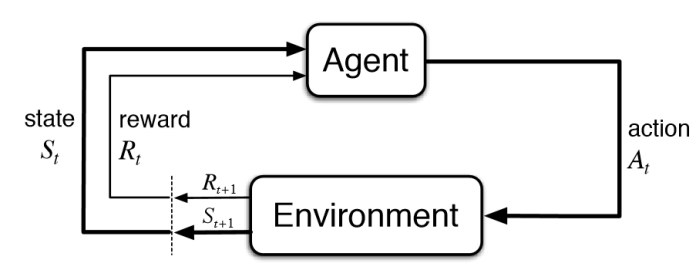
\includegraphics[]{figures/RL.jpg}
\caption[Reinforcement Learning]{Reinforcement Learning \protect\cite{Book.RLAI}}
\label{Fig.RL}
\end{figure}

\editnote{Types of environments}
Each environment can be assigned one of two characteristics from 7 categories:

\begin{itemize}
\item Fully observable vs. partially observable: If an agent have access to the complete state of the environment at each point in time, then we say that the environment is fully observable. An environment might be partially observable because of noisy and inaccurate observations or because parts of the state are simply not accessible for the agent e.g. an automated taxi cannot see what other drivers are thinking.
\item Single agent vs. multi-agent: The distinction between single-agent and multiagent environments may seem simple enough. For example, an agent solving a crossword puzzle by itself is clearly in a single-agent environment, whereas an agent playing chess is in a two-agent environment.
\item Deterministic vs. stochastic: If the next state of the environment is completely determined by the current state and the action executed by the agent, then we say the environment is deterministic. Otherwise, it is stochastic. If the environment is partially observable, however, then it could appear to be stochastic. Most real situations are so complex that it is impossible to keep track of all the unobserved aspects. For practical purposes, they must be treated as stochastic. It is often said that an environment is uncertain if it is not fully observable or not deterministic, because an agent can not be sure the outcomes of its actions.
\item Episodic vs. continuing: In an episodic environment, the agent’s experience is divided into episodes which finish at the terminal state. Crucially, the next episode does not depend on the actions taken in the previous episode. In continuing environments, on the other hand, the agent's experience may go on and on forever and there is no a distinct terminal state.
\item Static vs. dynamic: If the environment can change while an agent is deliberating, then we say the environment is dynamic for that agent. Otherwise, it is static.
\item Discrete vs. continuous: The discrete/continuous distinction applies to the internal state of the environment, to the way time is handled, and to the observations and actions of the agent. For example, the chess environment has a finite number of distinct states. Chess also has a discrete set of actions. Taxi driving is a continuous-state and continuous-time problem: the speed and location of the taxi and of the other vehicles sweep through a range of continuous values and do so smoothly over time. Taxi-driving actions are also continuous: steering angles, etc.
\item Known vs. unknown: Strictly speaking, this distinction refers not to the environment itself but to the agent’s (or designer’s) state of knowledge about the “laws of physics” of the environment. In a known environment, the outcomes, or outcome probabilities if the environment is stochastic, for all actions are given. It means that the agent have access to the environment's MDP. Obviously, if the environment is unknown, the agent will have to learn how it works in order to make good decisions.
\end{itemize}

\editnote{Dynamic Programming}
The term dynamic programming refers to a collection of algorithms that can be used to compute optimal policies given a perfect model of the environment as a Markov decision process (MDP). Classical dynamic programming algorithms are of limited utility in reinforcement learning both because of their assumption of a perfect model and because of their great computational expense, but they are still important theoretically. Dynamic programming provides an essential foundation for the understanding of the methods presented in this thesis. In fact, all of these reinforcement learning methods can be viewed as attempts to achieve much the same effect as dynamic programming, only with less computation and without assuming a perfect model of the environment.

First question to answer is: how to compute the state value function $V(s)$ for an arbitrary policy $\pi$? The process of doing so is called policy evaluation. It is easy to note that for all states $s$: $V_\pi(s) = \EX_\pi[G_t | s_t = s] = \EX_\pi[R_{t+1} + \gamma G_{t+1} | s_t = s] = \EX_\pi[R_{t+1} + \gamma V_\pi(s_{t+1}) | s_t = s]$, where the expectations are over the environment dynamics and are subscripted by $\pi$ to indicate that they are conditional on $\pi$ being followed. The existence and uniqueness of $V_\pi$ are guaranteed as long as either $\gamma < 1$ or eventual termination is guaranteed from all states under the policy $\pi$. If the environment’s dynamics are completely known, then the equation is a system of $|S|$, number of states, simultaneous linear equations in $|S|$ unknowns. In principle, its solution is a straightforward, if tedious, computation. For more practical purposes, iterative solution methods are available \cite{Book.RLAI}, but not described here.

Major reason for computing the value function for a policy is to help find better policies. With determined the value function $V_\pi$ for an arbitrary deterministic policy $\pi$, the question now is: if for some state $s$ changing the policy to deterministically choose an action $a \neq \pi(s)$, different then from the current policy, yields higher expected return? The value function tells how good it is to follow the current policy from $s$, but would it be better or worse to change to the new policy? One way to answer this question is to consider selecting $a$ in $s$ and thereafter following the existing policy $\pi$. The value of this way of behaving is $Q_\pi(s, a) = E[R_{t+1} + \gamma V_\pi(s_{t+1}) | s_t = s, a_t = a]$, where expectation is over the environment dynamics. The key criterion is whether this is greater than or less than $V_\pi(s)$. If it is greater — that is, if it is better to select $a$ once in $s$ and thereafter follow $\pi$ than it would be to follow $\pi$ all the time — then one would expect it to be better still to select $a$ every time $s$ is encountered, and that the new policy would in fact be a better one overall. It is a natural extension to consider changes at all states and to all possible actions, selecting at each state the action that appears best according to $Q_\pi(s, a)$ and this way create a new, improved policy: $\pi' = \underset{a}{\mathrm{argmax}}Q_\pi(s, a)$. The process of making a new policy that improves on an original policy, by making it greedy with respect to the value function of the original policy, is called policy improvement. If the new policy is as good as, but not better then, the old policy, then it is the optimal policy, which can be proved without much trouble \cite{Book.RLAI}.

Policy iteration consists of two simultaneous, interacting processes, one making the value function consistent with the current policy, policy evaluation, and the other making the policy greedy with respect to the current value function, policy improvement. In policy iteration, these two processes alternate, each completing before the other begins, but this is not really necessary. In value iteration, for example, only a single iteration of policy evaluation is performed in between each policy improvement. In asynchronous dynamic programming methods, the evaluation and improvement processes are interleaved at an even finer grain. In some cases a single state is updated in one process before returning to the other. As long as both processes continue to update all states, the ultimate result is typically the same: convergence to the optimal value function and an optimal policy. \\
The term generalized policy iteration is used to refer to the general idea of letting policy-evaluation and policy-improvement processes interact, independent of the granularity and other details of the two processes. Almost all reinforcement learning methods are well described as general policy iteration. That is, all have identifiable policies and value functions, with the policy always being improved with respect to the value function and the value function always being driven toward the value function for the improvement policy, as suggested by the fig.\ref{Fig.GPI}. If both the evaluation process and the improvement process stabilize, that is, no longer produce changes, then the value function and policy must be optimal \cite{Book.RLAI}.

\begin{figure}[H]
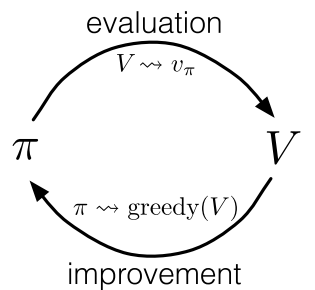
\includegraphics[width=0.4\textwidth,keepaspectratio]{figures/GPI.png}
\caption{General Policy Iteration \protect\cite{Book.RLAI}}
\label{Fig.GPI}
\end{figure}

\editnote{Credit assignment and exploration-exploitation problems}
Reinforcement learning faces two dilemmas. The first one is: How do you distribute credit for success among the many decisions that may have been involved in producing it? It is called credit-assignment problem, which past actions to reinforce for a positive outcome. \\
The second one is exploration-exploitation trade-off. To find a good policy, such that maximise an expected return, an agent needs to explore its options: if it would behave greedily all the time, it simply could not know if other actions lead to better returns. On the other hand, the agent also needs to exploit its knowledge about an environment in order to do well and progress in the environment to otherwise unavailable states. In other words, for policy evaluation to work, continual exploration needs to be assured. The most common approach to assuring that all state–action pairs are encountered is to consider only policies that are stochastic with a nonzero probability of selecting all actions in each state. \\
So called exploration policies are made to exploit an agent's knowledge about an environment, but at the same time, these constantly explore the environment's state-space. These policies are told to be soft, meaning that $\pi(a|s) > 0$ for every action in every state. One such family of policies is called $\epsilon$-greedy, meaning that most of the time they choose an action that has maximal estimated action value, but with probability $\epsilon$ they instead select an action at random. That is, all non-greedy actions are given the minimal probability of selection $\frac{\epsilon}{|A(s)|}$, where $|A(s)|$ is number of legal actions in state $s$, and the remaining bulk of the probability, $1 - \epsilon + \frac{\epsilon}{|A(s)|}$, is given to the greedy action. The bigger the $\epsilon$, the higher the exploration rate and vice versa.

\editnote{On-policy vs. Off-policy}
There are two general approaches to reinforcement learning: on-policy methods and off-policy methods. On-policy methods attempt to evaluate or improve the policy that is used to make decisions, whereas off-policy methods evaluate or improve a policy different from that used to generate the data. In the former case, an agent is extra sensitive to imperfect updates, in cases when its value function or its policy are somehow approximated. Because the agent learns directly from its behaviour, if the bad update makes the agent behave worse then before, the agent effectively falls back in its learning progress. Also, the on-policy methods learn action values not for the optimal policy, but for a near-optimal policy that still explores, which is required as noted before. \\
An example of on-policy algorithm would be Monte-Carlo control \cite{Book.RLAI}. Because it is reinforcement learning setting an agent do not have access to underlying MDP or POMDP and needs to learn from interactions with an environment, from its experience. An obvious way to an action value function learning, or policy evaluation, is simply to play with the environment using the current policy and average the returns observed after visits to each state-action pair. As more returns are observed, the average should converge to the expected value. Policy improvement is done by making the policy $\epsilon-$greedy with respect to the current value function. The two proceed according to the idea of generalized policy iteration.

In off-policy case, the behavioural exploratory policy is used for experience collection, which is then used to steadily improve the target policy towards the optimum. These methods, although favourable, are often more complex. Because the data is due to a different policy, off-policy methods are often of greater variance and are slower to converge. On the other hand, off-policy methods are more powerful and general. They include on-policy methods as the special case in which the target and behavior policies are the same. Off-policy methods also have a variety of additional uses in applications. For example, they can often be applied to learn from data generated by a conventional non-learning controller, or from a human expert. An example of off-policy algorithm would be Q-Learning \cite{Book.RLAI}, which is not described here.

\editnote{Model-free vs. Model-based}
There are two major kinds of reinforcement learning methods, model-free and model-based. Model-based methods rely on planning as their primary component, while model-free methods primarily rely on learning. The word planning is used in several different ways in different fields. In reinforcement learning the term is used to refer to any computational process that takes a model as input and produces or improves a policy for interacting with the modeled environment. \\
Although there are real differences between these two kinds of methods, there are also great similarities. In model-free reinforcement learning, the agent samples episodes of real experience and updates its value function from real experience. In model-based reinforcement learning the agent samples episodes of simulated experience and updates its value function from simulated experience. This symmetry between learning and planning has an important consequence: algorithms for learning can also become algorithms for planning, simply by substituting simulated experience in place of real experience.

The model of an environment can mean anything that an agent can use to predict how the environment will respond to its actions. Given a state and an action, a model produces a prediction of the resultant next state and next reward. If the model is stochastic, then there are several possible next states and next rewards, each with some probability of occurring. Some models produce a description of all possibilities and their probabilities. These are called distribution models. Other models produce just one of the possibilities, sampled according to the probabilities. These are called sample models. The kind of model assumed in dynamic programming, estimates of the MDP’s dynamics $P^a_{ss'}$ and $R^a_{ss'}$, is a distribution model. \\
Models can be used to mimic or simulate experience. Given a starting state and action, a sample model produces a possible transition, and a distribution model generates all possible transitions weighted by their probabilities of occurring. Given a starting state and a policy, a sample model could produce an entire episode, and a distribution model could generate all possible episodes and their probabilities. In either case,it is said that the model is used to simulate the environment or rollout the trajectory and produce simulated experience.

In artificial intelligence, there are two distinct approaches to planning according to the definition presented. State-space planning, which is viewed primarily as a search through the state-space for an optimal policy or an optimal path to a goal. Actions cause transitions from state to state, and value functions are computed over states. \\
In what is called plan-space planning, planning is instead a search through the space of plans. Operators transform one plan into another, and value functions, if any, are defined over the space of plans. Plan-space planning includes evolutionary methods.

Within a planning agent, there are at least two roles for real experience: it can be used to improve the model, to make it more accurately match the real environment, and it can be used to directly improve the value function and policy using the kinds of model-free reinforcement learning. The former is called model-learning, and the latter is called direct reinforcement learning. The possible relationships between experience, model, values, and policy are summarized in the fig.\ref{Fig.ModelBasedRL}. It can be seen, that experience can improve value functions and policies either directly or indirectly via the model. \\
Planning is often conducted in small, incremental steps. This enables planning to be interrupted at any time, which appears to be a key requirement for efficiently intermixing planning with acting and with learning of the model. Planning in very small steps may be the most efficient approach even in pure planning problems if the problem is too large to be solved exactly or the agent can not wait for exact solution and needs to act based on approximated one.

\begin{figure}[H]
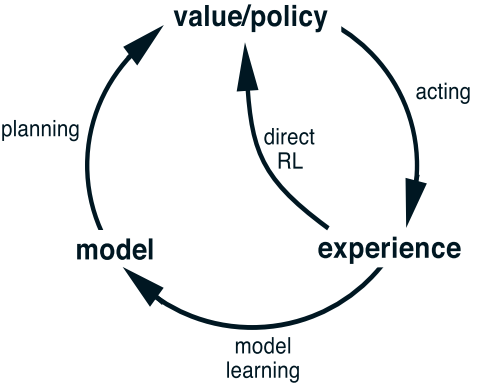
\includegraphics[width=0.4\textwidth,keepaspectratio]{figures/ModelBasedRL.png}
\caption{Model-based Reinforcement Learning. \protect\cite{Book.RLAI} Each arrow shows a relationship of influence and presumed improvement.}
\label{Fig.ModelBasedRL}
\end{figure}

\subsection{Simulation-Based Search}

Simulation-based search is something called planning at decision time \cite{Book.RLAI} and can be used, of course, in model-based reinforcement learning setting. It requires a sample model of the MDP, which can sample state transitions and rewards from $P^a_{ss'}$ and $R^a_{ss'}$ respectively. However, it is not necessary to know these probability distributions explicitly. The next state and reward could be generated by a black box simulator. The efficiency and effectiveness of simulation-based search depends in large part on the performance and accuracy of the model. The model learning problem is described later. Now, access to a perfect sample model is assumed.

Simulation-based search algorithms sample experience in sequential episodes. Each simulation begins in a root state $s_0$. At each step $u$ of simulation, an action $a_u$ is selected according to a simulation policy, and a new state $s_{u+1}$ and reward $r_{u+1}$ is generated by the sample model. This process repeats, without backtracking, until a terminal state is reached. The values of states or actions are then updated from the simulated experience. \\ Simulation-based search is usually applied online, at every time-step $t$, by initiating a new search that starts from the current state $s_0 = s_t$. The distribution of simulations then represents a probability distribution over future experience from time-step $t$ onwards. Simulation-based search exploits temporality, in other words focuses on the current situation, by learning from this specific distribution of future experience, rather than learning from the distribution of all possible experience. Furthermore, as the agent’s policy improves, the future experience distribution will become more refined. It can focus its value function on what is likely to happen next, given the improved policy, rather than learning about all possible eventualities.

Monte-Carlo simulation is a very simple simulation-based search algorithm for evaluating candidate actions from a root state $s_0$. The search proceeds by simulating complete episodes from $s_0$ until termination, using a fixed simulation policy. The action values $Q(s_0, a)$ are estimated by the mean outcome of all simulations with candidate action $a$.

Monte-Carlo tree search (MCTS) is perhaps the best-known example of a simulation-based search algorithm. It makes use of Monte-Carlo simulation to evaluate the nodes of a search tree. There is one node, $n(s)$, corresponding to every state $s$ encountered during simulation. Each node contains a total count of visits of the state, $N(s)$, a value $Q(s, a)$ and a visit count $N(s, a)$ for every possible action in a state $s$. Simulations start from the root state $s_0$, and are divided into two stages. When state $s_u$ is contained in the search tree, a tree policy selects the action with the highest value $Q(s, a)$. Otherwise, a random default policy is used to roll out simulations to completion. After each simulation, $s_0, a_0, r_1, s_1, a_1, ..., r_T$, each node $n(s_u)$ in the search tree is updated incrementally to maintain the count and mean return from that node,
$$N(s_u) \leftarrow N(s_u) + 1$$
$$N(s_u, a_u) \leftarrow N(s_u, a_u) + 1$$
$$Q(s_u, a_u) \leftarrow Q(s_u, a_u) + \frac{G_u - Q(s_u, a_u)}{N(s_u, a_u)}$$

\subsection{Deep Learning}

Machine learning gives AI systems the ability to acquire their own knowledge, by extracting patterns from raw data. It stands in opposition to classical computer programs which execute explicit instructions hand-coded by a programmer.
One example of machine learning algorithm is logistic regression. It can determine whether to recommend cesarean delivery or not \cite{Study.Cesarean}. Another widely used machine learning algorithm called naive Bayes can distinguish between legitimate and spam e-mail.

The performance of these machine learning algorithms depends heavily on the representation of the problem they are given. For example, when logistic regression is used to recommend cesarean delivery, the AI system does not examine the patient's MRI scan directly. It would not be able to make useful predictions as individual pixels in an MRI scan have negligible correlation with any complications that might occur during delivery. It, instead, gets several pieces of relevant information, such as the presence or absence of a uterine scar, from the doctor. Each piece of information included in the representation of the data is known as a feature. Logistic regression learns the relation between those features and various outcomes, such as a recommendation of cesarean delivery. The algorithm does not influence the way that the features are defined in any way.

Sometimes it can be hard to hand-craft a good problem's representation. For example, suppose that someone would like to write a program to detect cats in photographs. People know that cats are furry and have whiskers, so they might like to use the presence of a fur and whiskers as features. Unfortunately, it is difficult to describe exactly what a fur or a whisker looks like in terms of pixel values. This gets even more complicated when taking into account e.g. shadows falling on the cat or an object in the foreground obscuring part of the animal.
One solution to this problem is to use machine learning to discover not only the mapping from representation to output but also the representation itself. This approach is known as representation learning. Learned representations often result in much better performance of machine learning algorithms than can be obtained with hand-designed representations. They also allow AI systems to rapidly adapt to new tasks with minimal human intervention.

Deep learning is a particular kind of machine learning that achieves great power and flexibility by learning to represent the world as a nested hierarchy of concepts, with each concept defined in relation to simpler concepts. Deep learning solves representation learning problem by introducing representations that are expressed in terms of other, simpler representations. Fig.~\ref{Fig.DL} shows how a deep learning system can represent the concept of an image of a person by combining simpler concepts, such as corners and contours, which are in turn defined in terms of edges.

\begin{figure}[H]
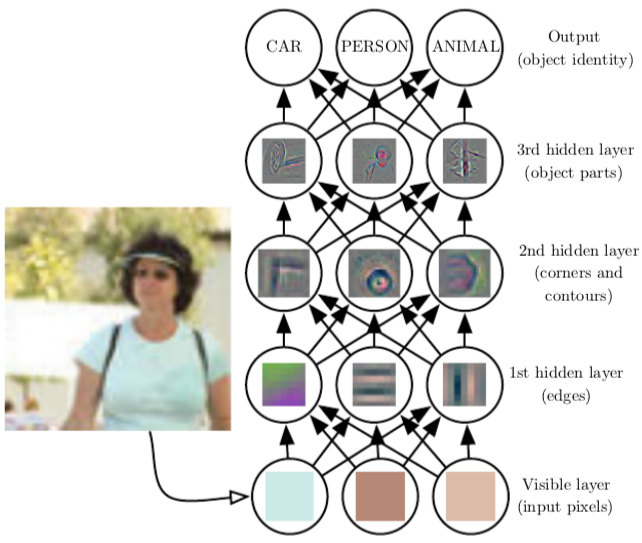
\includegraphics[width=0.8\textwidth,keepaspectratio]{figures/DL.png}
\caption[Deep Learning]{Deep Learning \protect\cite{Book.DeepLearning}}
\label{Fig.DL}
\end{figure}

The fundamental example of a deep learning model is a fully-connected (FC) neural network (NN), sometimes called a multilayer perceptron (MLP). A MLP is just a mathematical function mapping some set of input values to output values. The function is formed by composing many simpler functions, called neurons or perceptrons, into layers. Each layer provides a new representation of its input, which might be a vector, to all the neurons in the next layer by multiplying the input element-wise with its parameters and applying some kind of non-linear activation function to the sum of these products e.g. sigmoid function. Without the mentioned activation function, the multilayer NN would just simplify to a linear mapping without ability to model non-linear relationships of inputs and outputs of the NN. Fig.~\ref{Fig.MLP} shows example MLP and dependencies between perceptrons. The input is presented at the input layer. Then a hidden layer (or series of them) extracts increasingly abstract features from the image. These layers are called “hidden” because their values are not given in the data. Instead, the model must determine which concepts are useful for explaining the relationships in the observed data. Finally, this description of the input in terms of the features can be used to produce the output at the output layer.

\begin{figure}[H]
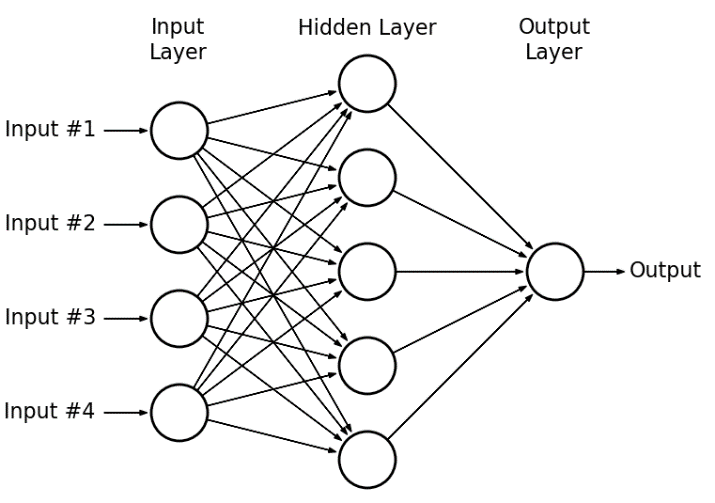
\includegraphics[width=0.8\textwidth,keepaspectratio]{figures/MLP.png}
\caption{Multilayer perceptron}
\label{Fig.MLP}
\end{figure}

Other type of very common neural network is a recurrent neural network (RNN). Humans do not start their thinking from scratch every second. As they read this thesis for example, they understand each word based on their understanding of previous words. Their thoughts have persistence. MLPs can not do this, that is why RNNs address this issue. These are networks with loops in them, allowing information to persist. In the fig.~\ref{Fig.RNN}, a chunk of neural network, $A$, looks at some input $x_t$ and outputs a value $h_t$. A loop allows information to be passed from one step of the network to the next. It turns out that RNNs are not all that different than a normal feedforward neural network. A recurrent neural network can be thought of as multiple copies of the same network, each passing a message to a successor.

\begin{figure}[H]
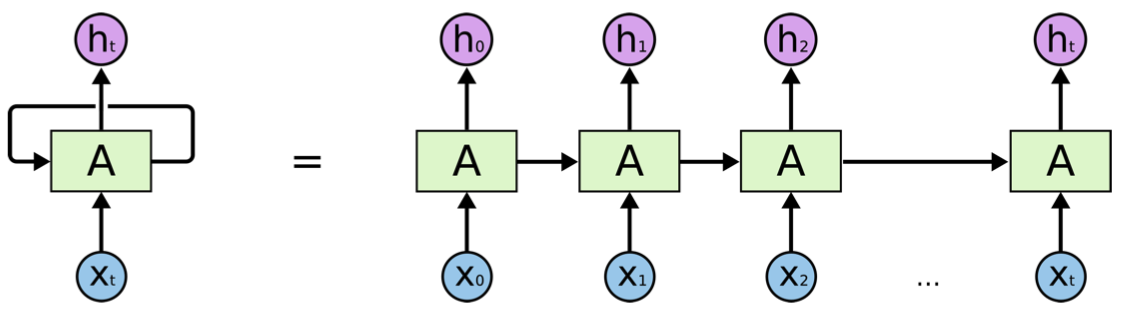
\includegraphics[width=0.8\textwidth,keepaspectratio]{figures/RNN.png}
\caption{A recurrent neural network \cite{Blog.RNNs}}
\label{Fig.RNN}
\end{figure}

Yet another very useful NN architecture is a convolutional neural network (CNN) which makes use of the fact that inputs to a NN can often have similar patterns in different parts of the input. For example in images, the object can appear in different positions in the image, but it is still the same object. CNNs exploit that fact by grouping parameters info filters in each layer and slide, or more precisely convolve, each filter across the width and height of the input volume and compute dot products between the entries of the filter and the input at any position. The 2D outputs of all filters are stacked together to form a 3D activation map. It is then processed by the next, similar, layer with its own set of filters. At the end of CNN, the final 3D volume is often flattened into a vector and then further processed by a fully-connected NN. The example CNN is shown in fig.~\ref{Fig.CNN}. \\
A CNN is able to successfully capture the spatial dependencies in an image through the application of relevant filters. The architecture performs a better fitting to the data with spatial hierarchy due to the reduction in the number of parameters involved and reusability of weights.

\begin{figure}[H]
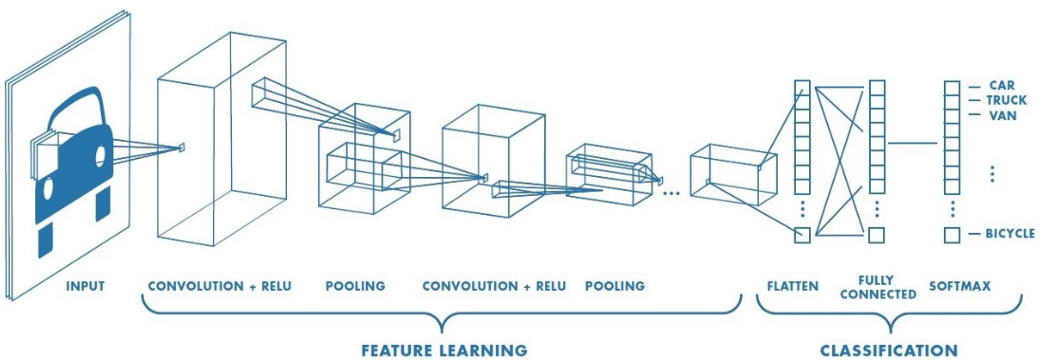
\includegraphics[width=0.9\textwidth,keepaspectratio]{figures/CNN.png}
\caption{A convolutional neural network \cite{Blog.CNNs}. ReLU \cite{Algo.ReLU} and Softmax are activation functions. Pooling means that each filter's output is divided into, for instance, 2 x 2 regions and only maximum value from each region is passed to the next layer.}
\label{Fig.CNN}
\end{figure}

A neural network is trained, in the simplest case, to output a correct target value for each input from a dataset. This is done by backpropagating some measure of error, how much different is the NN's output value from the target value, through the NN. This produces gradients. Gradients are vectors that point in the direction of steepest ascent of the NN's error. These are used in the opposite direction to iteratively change parameters and lower the error on the dataset. The process is repeated iteratively, updates are small steps, because gradients are first order derivatives and the directions these point in are accurate only locally. This algorithm is called gradient decent (GD) and it is at the heart of the deep learning. More about neural networks and training procedures can be found in the Deep Learning book \cite{Book.DeepLearning}.

\subsection{Variational Inference}
\editnote{TODO: Describe vanilla VAEs and VAEs in structured POMDPs (filtering).}
 \newpage
\section{State of the art}

\subsection{World Models}

\editnote{High-level idea or abstract.} In World Models \cite{Algo.WorldModels} paper, its authors explore the idea of using large and highly expressive neural networks, that can learn rich spatial and temporal representation of data, and applying them to reinforcement learning. The RL algorithm is often bottlenecked by the credit assignment problem, which makes it hard for traditional RL algorithms to learn millions of weights of a large model. To accomplish their goal, they decompose the problem of an agent training into two stages: they first train a generative neural network to learn a model of the agent's world in an unsupervised manner. Thereafter, by using a compressed spatial and temporal representation of the environment extracted from the world model as inputs to the agent, they train a linear model to learn to perform a task in the environment. The small linear model lets the training algorithm focus on the credit assignment problem on a small search space, while not scarifying capacity and expressiveness via the larger world model.

Their solution consists of three components: Vision for encoding the spatial information, Memory for encoding the temporal information and Controller which represents the agent's policy. Fig.~\ref{Fig.WorldModels} depicts a flow diagram of the agent's model.

\begin{figure}[H]
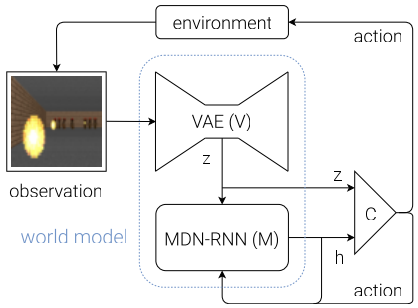
\includegraphics[width=0.7\textwidth,keepaspectratio]{figures/WorldModels.png}
\caption[Flow diagram of the World Models agent's model]{Flow diagram of the agent's model \protect\cite{Algo.WorldModels}. The raw observation is first processed by the Vision at each time step $t$ to produce $z_t$. The input into the Controller is this latent vector $z_t$ concatenated with the Memory hidden state $h_t$ at each time step. The Controller will then output an action vector $a_t$ and will affect the environment. The Memory will then take the current $z_t$ and action $a_t$ as an input to update its own hidden state to produce $h_{t+1}$ to be used at time step $t + 1$.}
\label{Fig.WorldModels}
\end{figure}

The environment provides the agent with high dimensional visual observation at each time step. The essential task of the Vision model is to encode this high dimensional observation into a low dimensional latent state. To do this, Vision is implemented as Variational Autoencoder \cite{Algo.VAE}. It is trained in an unsupervised manner on randomly generated experience from the environment. The authors assume that the random agent can efficiently explore environment and no iterative training procedure is implemented. The dataset is gathered once and fixed for Vision and Memory training.

Since many complex environment are partially observable, the visual observation at each time step, and hence the latent state, doesn't include full information about the current situation in the environment. To acquire full knowledge, the agent needs to encode what happens over time. This is the role of the Memory. It is implemented as popular recurrent neural network (RNN) architecture called Long Short-Term Memory \cite{Algo.LSTM} and trained on the same data as Vision to predict the next step future latent state that Vision is expected to produce. Because many environments are stochastic in nature, the RNN is trained to output a probability density of the next latent state approximated as a mixture of Gaussian distribution - in literature, this approach is known as Mixture Density Network combined with a RNN \cite{Algo.MDNRNN} (MDN-RNN). Moreover, using the stochastic Memory the authors are able to train more robust Controller, more on that later. \\
To be more precise, the MDN-RNN will model $p(z_{t+1} | o_{\leqslant t}, a_{\leqslant t}) = p(z_{t+1} | h_t) \prod_{i=1}^t q(z_i | o_i)$, where $h_t = f(h_{t-1}, z_t, a_t)$ is the hidden state of the RNN, $f$, that encodes past information about states and actions from the beginning of the episode until the time step $t$. Furthermore, $o_{t}$, $z_{t}$ and $a_{t}$ are the observation, the latent state and the action at time step $t$ respectively. During sampling they can adjust a temperature parameter $\tau$, that scale mixing coefficients in the MDN, to control model uncertainty \cite{Algo.Sketch-RNN}. They find it useful for training the Controller later on.

The Controller model represents the agent's policy. It is responsible for determining course of actions to take in order to solve a given task. Controller is a simple linear model that maps the concatenated latent state $z_t$ and hidden state $h_t$ at the time step $t$ directly to the action $a_t$ at that time step: $a_t = W[z_t h_t] + b$, where $W$ and $b$ are the weight matrix and bias vector of that model.
The authors deliberately made Controller as simple as possible, and trained it separately from Vision and Memory, so that most of the agent's complexity resides in the world model (V and M). The latter can take the advantage of current advances in deep learning that provide tools to train large models efficiently when well-behaved and differentiable loss function can be defined.
Shift in the agent's complexity towards the world model allows the Controller model to stay small and focus its training on tackling the credit assignment problem in challenging RL tasks. It is trained using evolution strategy, which is rather an unconventional choice that only currently have been considered as a viable alternative to popular RL techniques \cite{Algo.ESRL}.

\editnote{Main contributions or where it's SoTa.} Their solution is able to solve an OpenAI Gym's CarRacing environment \cite{Code.OpenAIGym}, which is the continuous-control, top-down racing task. It is the first known solution to achieve the score required to solve this task. In the process, the Memory model learns to simulate the original environment. The authors show that the learned Controller can function inside of the imagined environment of CarRacing, that is simulated by the Memory.
In the second experiment, they show that the agent is able to learn solely from imagined experience, produced by its Memory, and successfully transfer this policy back to the actual environment of VizDoom (see fig.~\ref{Fig.VizDoom}). In the first trials, the Controller learned to exploit imperfect simulations of the Model, which only approximates the true environment dynamics. To mitigate this behaviour, they adjust the temperature parameter of MDN-RNN to control the amount of randomness in the Memory, hence controlling the trade-off between realism and exploitability.

\begin{figure}[H]
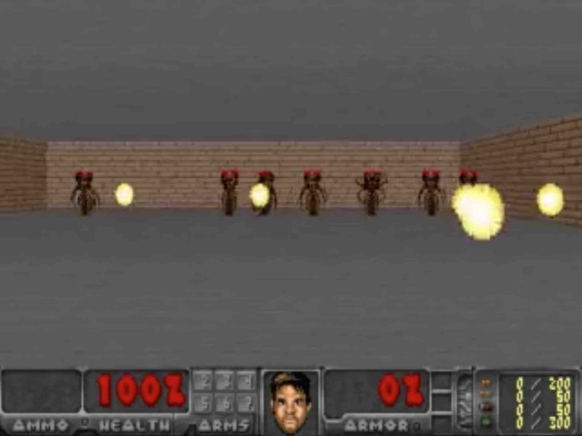
\includegraphics[width=0.7\textwidth,keepaspectratio]{figures/VizDoom.png}
\caption[VizDoom]{VizDoom: the agent must learn to avoid fireballs shot by monsters from the other side of the room with the sole intent of killing the agent \protect\cite{Algo.WorldModels}.}
\label{Fig.VizDoom}
\end{figure}

\editnote{Argument why and how (or not) you base on this work.} The authors results indicate that their world model is able to model complex environments from visual observations and it can be used for planning. Therefore, it may prove useful for the topic of this thesis.

\subsection{Learning Latent Dynamics for Planning from Pixels}

\editnote{High-level idea or abstract.}

\editnote{Main contributions or where it's SoTa.}

\editnote{Argument why and how (or not) you base on this work.}
 \newpage
\section{Planning with learned model}

In this section two architectures are described. Both involve a similar model learning approach, but differ substantially in technical details and planning algorithms. Both architectures use computationally efficient latent space environment models that make predictions at a higher level of spatial abstraction, than at the level of raw pixel observations. Such models substantially reduce the amount of computation required to make predictions, as future states can be represented much more compactly. In order to increase model accuracy and robustness, both models explicitly model uncertainty in state transitions using stochastic nodes. \cite{Algo.FastGenerativeModels}
The goal for both architectures stays the same: train a sufficiently accurate latent space environment's dynamics model, or such that accurately predicts future latent states and rewards to predefined cut-off point in time, and use it to plan and solve the environment. 
Before all of that, the code architecture and the framework that was created to accelerate this research are described.

\subsection{HumbleRL framework}

Reinforcement Learning scientists tend to write the entire code from scratch by themselves, instead of using existing RL frameworks. This is justified by the fact, that the commonly available frameworks are not flexible enough for intended experiments or require a specific backend like TensorFlow, which might be disfavored.
HumbleRL \cite{Code.HRL} was created with this problem in mind. Its simple API allows to perform a variety of RL experiments without any restrictions on the algorithms used. Since the backend is not tied to any specific technology, it is possible to mix different neural network frameworks or not use them at all. HumbleRL provides the boilerplate code of RL loop in fig.\ref{Fig.RL} and determines the common interfaces between an agent and an environment, the rest is designed by the user.

\subsubsection{Architecture}

Framework architecture is depicted in fig. \ref{Fig.HRL_architecture}. An agent is represented by the Mind class. The Mind encapsulates action planning logic and provides it via the plan method. In order to learn, the agent acts in the world represented by the Environment class. The Environment provides methods for resetting, taking steps, rendering and getting information about the world. The framework includes a factory function that creates and returns e.g. wrapped OpenAI Gym environment. The agent is not usually presented with raw environment observations. Instead, it looks at states preprocessed by the Interpreter. Different interpreters can be joined together with the ChainInterpreter class. It acts as a preprocessing pipeline, with each subsequent interpreter using the output of a previous one as an input.

\begin{figure}[H]
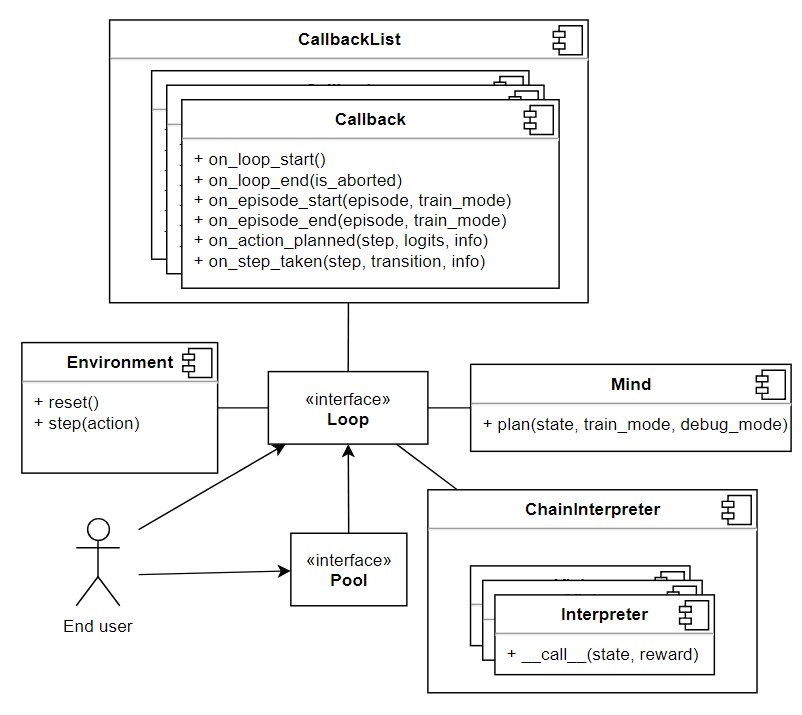
\includegraphics[width=0.6\textwidth,keepaspectratio]{figures/HumbleRL/architecture.png}
\caption{HumbleRL architecture}
\label{Fig.HRL_architecture}
\end{figure}

Framework user does not need to call all of those methods directly, those are utilized by the loop function. This function gets an action from the Mind, executes it in the Environment and then next observation is preprocessed with the Interpreter in preparation for the next step. To extend basic loop functionality, user can define callbacks that implement the Callback interface. Callbacks can react to events:
\begin{itemize}
\item at the beginning and ending of the loop,
\item at the beginning and ending of each episode,
\item after action is planned by the Mind,
\item after step is taken in the Environment.
\end{itemize}
Callbacks are accumulated in the CallbackList. The entire loop function logic is shown in fig. \ref{Fig.HRL_loop}.
Parallel version of loop function is available as the pool function. It uses predefined number of workers to execute a pool of Minds in their own Environments in parallel.

\begin{figure}[H]
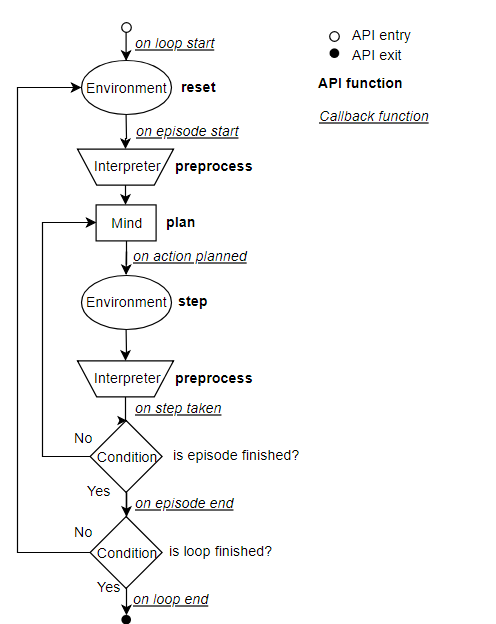
\includegraphics[width=0.6\textwidth,keepaspectratio]{figures/HumbleRL/loop.png}
\caption{HumbleRL loop function overview}
\label{Fig.HRL_loop}
\end{figure}

World Models with the AlphaZero planner uses this framework.

\subsection{World Models with the AlphaZero planner}

World Models' agent \cite{Algo.WorldModels} successfully plans using a learned model where the model is used to generate simulated experience on which the policy is trained. This section describes attempt to adjust and utilize the world model part of the agent in the AlphaZero search algorithm. This is different application of the model than in the original paper, where only future latent states and done flag are predicted, and therefore the model needs to be extend with a reward predictor and the controller is replaced by AlphaZero.

\subsubsection{World Models architecture: Vision and Memory}

A simple model inspired by human cognitive system is used. In this model, an agent has a visual sensory module that compresses observations into a small representative code. It also has a memory module that makes predictions about future codes based on historical information. Finally, the agent has a decision-making component that decides what actions to take based only on the representations created by its vision and memory modules. It uses AlphaZero and is described in the next section in details. \\
This architecture allows for training of a large neural network to tackle RL tasks by dividing the agent into a large world model and a small controller model. First a large neural network learns to model the agent’s world in an unsupervised manner, and only then the smaller controller focuses on the credit assignment problem on a smaller search space of controller's parameters, while not sacrificing capacity and expressiveness via the larger world model.

An environment provides the agent with a high dimensional input observation at each time step. It is a 2D image frame that is part of a video sequence. The vision module role, as already mentioned, is to learn an abstract representation of each observed input frame. It uses a simple Variational Autoencoder \cite{Algo.VAE} and, the same as in the original work described in the related work chapter, is trained to encode each frame into low dimensional latent vector by minimizing the difference between a given frame and the reconstructed version of the frame produced by the decoder. \\
The Memory module purpose is to compress the information what happens over time in its hidden state and enable simulation of the environment. To do this, it is trained to model environment's dynamics, predicting a future latent state from history of previous latent states, as a mixture of Gaussians. It models latent states with probability distribution to model uncertainty in the environment, but also create more robust environment's representation \cite{Algo.FastGenerativeModels}. Uncertainty can originate not only from fundamental stochastic nature of the environment, but also partial observability. \\
The model is implemented as a recurrent neural network with the Mixture Density Network (MDN) on top of a RNN's hidden state. In literature this architecture is called MDN-RNN \cite{Algo.MDNRNN}.

Figure \ref{Fig.WorldModelsPGM} depicts the world model, the Vision and Memory modules interconnection, in graphical form. More specifically, the world model components are:
\begin{itemize}
\item Deterministic hidden state model:      $h_t = f(h_{t-1}, z_{t}, a_{t})$
\item Stochastic latent state model:         $z_{t+1} \sim p(z_{t+1}|h_t) = \sum_c\pi_c(h_t)p(z_{t+1}|h_t, c)$
\item Observation model (decoder):           $o_t \sim p(o_t|z_t)$
\item Approximate state posterior (encoder): $z_t \sim q(z_t|o_t)$
\end{itemize}
where $o$, $z$ and $a$ are high-dimensional observations, latent states and actions respectively. $f(h_{t-1}, z_{t}, a_{t})$, the hidden state model, is implemented as a recurrent neural network and $h_t$ is its hidden state. The latent state model is a mixture of Gaussians with mean and variance parameterised by a feed-forward neural network. $c$ is a mixture's component and $\pi(h)$ is a normalized vector of mixing coefficients as a function of the RNN's hidden state. The observation model is Bernoulli distribution parameterised by a deconvolutional neural network. Since the model is non-linear, directly computing the state posteriors is intractable. Instead, an encoder $q$ is used to infer approximate state posteriors from past observations and actions, where $q(s_t | h_t, o_t)$ is a diagonal Gaussian with mean and variance parameterised by a convolutional neural network followed by a feed-forward neural network.

\begin{figure}[H]
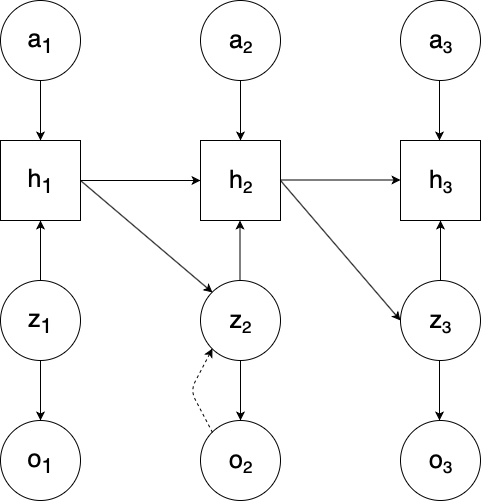
\includegraphics[width=0.45\textwidth,keepaspectratio]{figures/WorldModels/prob_graph_model.png}
\caption[World Models probabilistic graphical model]{World Models probabilistic graphical model: solid arrows describe the predictive model, dotted arrow describes the inference model, stochastic nodes are circles and squares depict deterministic nodes.}
\label{Fig.WorldModelsPGM}
\end{figure}

Because benchmarks include only deterministic environments and AlphaZero in its original form can only work with a deterministic dynamics model, this architecture in final experiments use the Memory module without the MDN and with a linear model instead. In fact, it uses two linear models to output the next latent state and reward.
\begin{itemize}
\item Deterministic hidden state model:      $h_t = f(h_{t-1}, s_{t}, a_{t})$
\item Deterministic latent state model:      $z_{t+1} = f(h_t)$
\item Deterministic reward model:            $r_{t+1} = f(h_t)$
\item Observation model (decoder):           $o_t \sim p(o_t|z_t)$
\item Approximate state posterior (encoder): $z_t \sim q(z_t|o_t)$
\end{itemize}
where $f$ in the latent state model and the reward model are the linear models.

HumbleRL is used to implement the original World Models architecture from the paper. This allows for easy adjustments for experiments purposes and to couple the world model with AlphaZero implementation in HumbleRL. An agent exploring an environment (Mind) and a callback are used to gather transitions and save them to an external storage. The framework allows to focus strictly on collecting trajectories and not worry about agent-environment interactions. \\
Collected transitions are used to train the Vision and Memory components. For Vision training Keras \cite{Code.Keras} framework is used. For Memory training PyTorch \cite{Code.PyTorch} framework is used, since it is easier to work with recurrent neural networks than in Keras. HumbleRL is not constricted to work with any particular deep learning library, so it is not a problem to mix the solutions, as long as trained models are wrapped in HumbleRL's interfaces. \\
The popular LSTM architecture \cite{Algo.LSTM} implements the Memory module RNN with 256 hidden units. The MDN is composed of 5 16-dimensional Gaussians with mean and log standard deviation parameterised by one layer feed-forward neural networks with linear activations. The Vision module neural networks are convolutional and deconvolutional neural networks shown in figure \ref{Fig.WorldModelsVAEArchitecture}.
The Vision module is trained using the Adam optimizer \cite{Algo.Adam} with a learning rate of $10^{-3}$ and $\epsilon = 10^{−7}$ on batches of 256 images. The Memory module is trained using the Adam optimizer \cite{Algo.Adam} too with a learning rate of $10^{-3}$ and $\epsilon = 10^{−8}$ on batches of 128 sequence chunks of length 1000.

\begin{figure}[H]
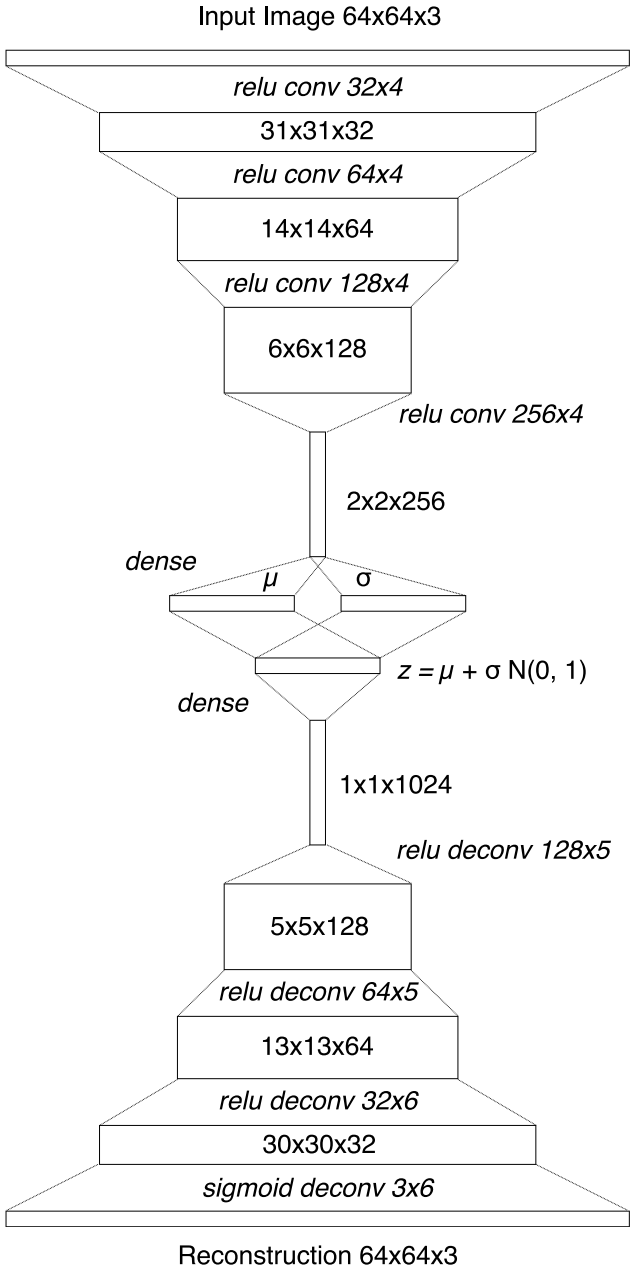
\includegraphics[width=0.45\textwidth,keepaspectratio]{figures/WorldModels/world_models_vae_architecture.png}
\caption{World Models VAE neural network architecture \cite{Algo.WorldModels}}
\label{Fig.WorldModelsVAEArchitecture}
\end{figure}

\subsubsection{AlphaZero architecture: Controller}

\editnote{TODO: Add a paragraph below about an AlphaZero backup phase modification to take into account rewards along the path.}

AlphaZero is composed from three main components: MCTS-like search algorithm, value and policy networks. The search algorithm itself is described in the related work chapter and doesn't change here. The value and policy networks are two linear models. 
The AlphaZero controller uses the world model for simulations. The Vision module is used as the Interpreter which encodes incoming observations into latent space. The Memory module, wrapped in the MDP interface from HumbleRL, is used in the expansion phase of AlphaZero. The Mind class, which is implemented by the AlphaZero algorithm, returns actions' scores. These are actions visit counts from the root state node, which are then used to choose an action by a policy. During training actions are sampled with probability proportional to these visit counts for fixed number of warm-up steps at the beginning of each episode to enhance exploration and after warm-up a greedy policy is used. During testing always greedy policy is used, which picks an action which was visited most often.
Pseudo-code written in Python of the search algorithm in the Mind is shown below:

\noindent\begin{minipage}{\textwidth}
\begin{lstlisting}[language=Python]
def plan(self, state):
    # Get/create root node
    root = self.query_tree(state)

    # Perform simulations
    simulations = 0
    start_time = time()
    while time() < start_time + self.timeout and simulations < self.max_simulations:
        # Simulate
        simulations += 1
        leaf, path = self.simulate(root)

        # Expand and evaluate
        value = self.evaluate(leaf)

        # Backup value
        self.backup(path, value)

    # Get actions' visit counts
    actions = np.zeros(self.model.action_space.num)
    for action, edge in root.edges.items():
        actions[action] = edge.num_visits

    return actions
\end{lstlisting}
\end{minipage}

The agent's experience and score statistics used for training are gathered using callbacks during the self-play phase. Maximum of 1000 games are kept. The neural network training phase takes place after 10 self-play games and lasts for 5 epochs. The training phase is performed using the Keras \cite{Code.Keras} framework. Next, the self-play phase takes place once again to gather new experience and the two further interchange until convergence. This architecture iteratively improves the AlphaZero's networks during training and then evaluate them collecting new data during self-play, which form a policy iteration framework.

\subsubsection{Data collection}

To train Vision and Memory modules first collection of 10,000 random rollouts of the environment are gathered to create a dataset. An agent is acting randomly to explore the environment multiple times and records the random actions taken and the resulting observations from the environment.
This dataset is used to train the Vision module. Next, it is used to process each frame into its latent state to prepare a dataset for the Memory module training, which works entirely in the latent space.
AlphaZero needs to collect its own data during training as it trains on-policy.

\subsubsection{Preprocessing}

Each frame, before it is used for any training, is central cropped if a frame from an environment includes some kind of border which doesn't inform an agent in anyway. This operation depends on a specific environment. It is then resized to 64 x 64 pixels for all environments. All three colour channels are preserved. Actions are one-hot encoded and default 4 action repeat from OpenAI Gym \cite{Code.OpenAIGym} is used as common in reinforcement learning \cite{Algo.DQN} to reduce the planning horizon and provide a clearer learning signal to the model.

\subsection{PlaNet with the CEM planner}

PlaNet (Deep Planning Network) \cite{Algo.PlaNet} shows working example of a planning agent that searches for the best sequence of future actions using a learned model in continuous control tasks. This is close to what this work tries to accomplish, but for a different type of environments. This section describe how it was utilized in episodic discrete tasks.

\subsubsection{RSSM architecture}

This architecture uses recurrent state space model (RSSM) which is similar to what World Models does. This latent dynamics model is designed with both deterministic and stochastic components \cite{Algo.FastGenerativeModels}. Original experiments indicate having both components to be crucial for high planning performance. It also uses a generalized variational bound that include multi-step predictions. Using only terms in latent space results in a fast regularizer that can improve long-term predictions. For more see related work. \editnote{QUESTION: Such cross-reference is legit?}

The same as in World Models, the model is provided with image observations. It even uses the same Variational Autoencoder with the same neural network architecture to encode the observations into latent space. The difference lies in the dynamics model shown in figure \ref{Fig.PlaNetPGM} with following components:
\begin{itemize}
\item Deterministic hidden state model:      $h_t = f(h_{t-1}, s_{t-1}, a_{t-1})$
\item Stochastic latent state model:         $s_t \sim p(s_t|h_t)$
\item Observation model (decoder):           $o_t \sim p(o_t|h_t, s_t)$
\item Reward model:                          $r_t \sim p(r_t|h_t, s_t)$
\item Approximate state posterior (encoder): $s_t \sim q(s_t|o_{\leqslant t}, a_{< t}) = \prod_{i=1}^tq(s_t|h_t,o_t)$
\end{itemize}
where $o$, $s$ and $a$ are high-dimensional observations, latent states and actions respectively. $f(h_{t-1}, s_{t-1}, a_{t-1})$, the deterministic state model, is implemented as a recurrent neural network and $h_t$ is its hidden state. The latent state model is Gaussian with mean and variance parameterised by a feed-forward neural network, the observation model is Gaussian with mean parameterised by a deconvolutional neural network and identity covariance, and the reward model is a scalar Gaussian with mean parameterised by a feed-forward neural network and unit variance. Since the model is non-linear, directly computing the state posteriors is intractable. Instead, an encoder $q$ is used to infer approximate state posteriors from past observations and actions, where $q(s_t | h_t, o_t)$ is a diagonal Gaussian with mean and variance parameterised by a convolutional neural network followed by a feed-forward neural network.

\begin{figure}[H]
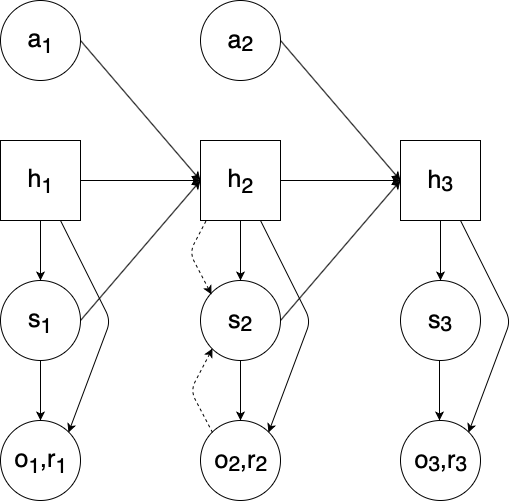
\includegraphics[width=0.45\textwidth,keepaspectratio]{figures/PlaNet/prob_graph_model.png}
\caption[World Models probabilistic graphical model]{PlaNet probabilistic graphical model: solid arrows describe the predictive model, dotted arrow describes the inference model, stochastic nodes are circles and squares depict deterministic nodes.}
\label{Fig.PlaNetPGM}
\end{figure}

\noindent There are two deviations from the World Models architectures:
\begin{itemize}
\item Hidden states are ``shifted'' to the right, so the previous state and action are used to predict the current hidden state $h$ and it is then used to predict the current latent state $s$.
\item VAE's decoder and encoder (named Vision in World Models) use the dynamics model's hidden state for prediction and inference. This way the likelihood and the posterior are conditioned on past observations too, as opposed to World Models.
\end{itemize}

Intuitively, this model can be understood as splitting the state into a stochastic part and a deterministic part, which depend on the stochastic and deterministic parts at the previous time step through the RNN. Importantly, all information about the observations must pass through the sampling step of the encoder to avoid a deterministic shortcut from inputs to reconstructions.

This time official code from repository \cite{Code.PlaNet} was adjusted and used for experiments. The code architecture follows principles from other PlaNet author's paper \cite{Code.TFAgents}.
The RSSM uses a GRU \cite{Algo.GRU} with 200 units as deterministic path in the dynamics model and implements all other functions as two fully connected layers of size 200 with ReLU activations \cite{Algo.ReLU}. Distributions in latent space are 30-dimensional diagional Gaussians with predicted mean and standard deviation.
The observation model and the approximate state posterior are implemented with the Variational Autoencoder, the same as in World Models (see fig.\ref{Fig.WorldModelsVAEArchitecture}). The reward model is implemented with a feed-forward neural network with two hidden layers of size 100.
The model is trained jointly using the Adam optimizer \cite{Algo.Adam} with a learning rate of $10^{-3}$ and $\epsilon = 10^{−4}$, and gradient clipping norm of 1000 on batches of 50 sequence chunks of length 50. The KL divergence terms are also scaled relatively to the reconstruction terms and the model is granted free nats by clipping the divergence loss below this value. Both parameters are tuned in experiments chapter. Latent overshooting from the paper \cite{Algo.PlaNet} is used with overshooting KL divergence terms additionally scaled by a factor of $1/50$.

\subsubsection{CEM planner}

The agent plans using the cross entropy method (CEM) \cite{Algo.CEM} to search for the best action sequence under the model, the same as in the PlaNet. CEM is a population-based optimization algorithm that infers a distribution over action sequences that maximize the objective.
First, a time-dependent diagonal Gaussian belief over optimal action sequences gets initialized: $a_{t:t+H} \sim Normal(\mu_{t:t+H}, \sigma^2_{t:t+H}I)$, where $t$ is the current time step of the agent and $H$ is the length of the planning horizon (12 by default). Starting from zero mean and unit variance, 1000 candidate action sequences are sampled and evaluated under the learned model. Then the belief gets re-fitted to the top 100 action sequences. After 10 iterations, the planner returns the mean of the belief for the current time step $\mu_t$ which is then used by the policy to choose discrete action. Importantly, after receiving the next observation, the belief over action sequences starts from zero mean and unit variance again to avoid local optima. \\
When collecting episodes for the training data set the epsilon greedy policy is used with $\epsilon = 0,3$. During test phase the greedy policy is used, which chooses the action that maximises the returned belief. \\
To evaluate a candidate action sequence under the learned model, a trajectory starting from the current state is sampled and the predicted rewards are summed along the sequence. Since it is a population-based optimizer,
it is sufficient to consider a single trajectory per action sequence and thus focus the computational budget on evaluating a larger number of different sequences. Because the reward is modeled as a function of the latent state, the planner can operate purely in latent space without generating images, which allows for fast evaluation of large batches of action sequences.

\editnote{TODO: Add algorithm of planning procedure.}

\subsubsection{Data collection}

Since the agent may not initially visit all parts of the environment, new experience needs to be iteratively collect and then the dynamics model gets refined. It is done so by planning with the partially trained model. Starting from a small amount of 6 seed episodes collected under random actions, the model is trained and one additional episode is added to the data set every 5000 update steps.

\subsubsection{Preprocessing}

Each image gets preprocessed by reducing the bit depth to 5 bits as in \cite{Algo.Glow5bit}. It is then resized to 64 x 64 pixels for all environments.
Actions are one-hot encoded and each action gets repeated 4 times as common in reinforcement learning \cite{Algo.DQN} to reduce the planning horizon and provide a clearer learning signal to the model.
 \newpage
\section{Experiments}

\subsection{Benchmarks}

\subsubsection{Arcade Learning Environment}

The Arcade Learning Environment (ALE) has became a platform for evaluating artificial intelligence agents. Originally proposed by Bellemare et. al. \cite{Code.ALE}, the ALE makes available dozens of Atari 2600 games for an agent training and evaluation. The agent is expected to do well in as many games as possible without game-specific information, generally perceiving the world through a video stream. Atari 2600 games are excellent environments for evaluating AI agents for three main reasons: they are varied enough to provide multiple different tasks, requiring general competence, they are interesting and challenging for humans and they are free of experimenter’s bias, having been developed by an independent party.

In the context of the ALE, a discrete action is a number in range from 0 to 17 inclusive which encodes the composition of a joystick direction and an optional button press. The agent observes a reward signal, which is typically the change in the player’s score (the difference in score between the previous time step and the current time step), and an observation $o_t \in O$ of the environment. This observation can take form of a single 210 × 160 image and/or the current 1024-bit RAM state. Because a single image typically does not satisfy the Markov property the ALE is formalised as POMDP. Observations and the environment state are distinguished, with the RAM data being the real state of the emulator. A frame (as a unit of time) corresponds to 1/60th of a second, the time interval between two consecutive images rendered to the television screen. The ALE is deterministic, which means that given a particular emulator state $s$ and a action $a$ there is a unique next state $s'$, that is, $P^a_{ss'} = p(s' | s, a) = 1$.

Agents interact with the ALE in an episodic fashion. An episode begins by resetting the environment to its initial configuration, $s_0$, and ends at a given endpoint depending on a game. The primary measure of an agent’s performance is the score achieved during an episode, namely the undiscounted sum of rewards for that episode. While this performance measure is quite natural, it is important to realize that score is not necessarily an indicator of AI progress. In some games, agents can exploit the game's mechanics to maximize sum of rewards, but not complete the game's goal in human's understanding. \cite{Study.FaultyReward}

Preprocessing include frame skipping \cite{Study.FrameSkipping} which restricts the agent’s decision points by repeating a selected action for 4 consecutive frames. Frame skipping results in a simpler reinforcement learning problem and speeds up execution.
\editnote{TODO: Describe other preprocessing techniques used here.}

This work uses ALE through OpenAI Gym API \cite{Code.OpenAIGym}, specifically two games are used as benchmarks: Boxing and Freeway.

Boxing is a video game based on the sport of boxing. Boxing shows a top-down view of two boxers, one white and one black. When close enough, a boxer can hit his opponent with a punch. This causes his opponent to reel back slightly and the boxer scores a point, a reward of 1. In the other situation, when the boxer gets hit, he gets a negative reward of -1. There are no knockdowns or rounds. A match is completed either when one player lands 100 punches (a 'knockout') or two minutes have elapsed. In the case of a decision, the player with the most landed punches is the winner. Ties are possible. 
While the gameplay is simple, there are subtleties, such as getting an opponent on the 'ropes' and 'juggling' him back and forth between alternate punches. 

\begin{figure}[H]
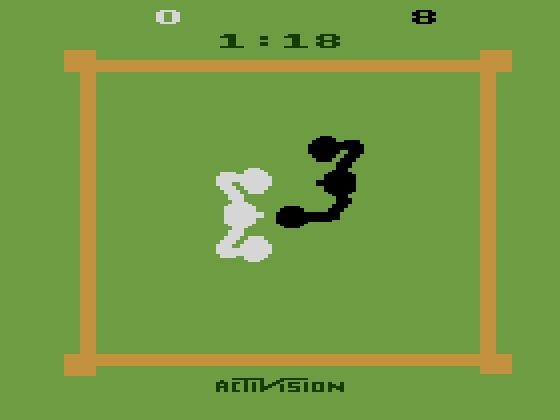
\includegraphics[width=0.5\textwidth,keepaspectratio]{figures/Boxing.jpg}
\caption[Sokoban]{Example of Boxing level}
\label{Fig.Boxing}
\end{figure}

In Freeway an agent controls a chicken who can be made to run across a ten lane highway filled with traffic in an effort to 'get to the other side.' Every time a chicken gets across a reward of 1 is earned by the agent. If hit by a car, then a chicken is forced back slightly. The goal is to score as much points as possible in the two minutes. The chicken is only allowed to move up or down. 
The major challenge in this environment are sparse rewards. The agent scores only when successfully crosses the highway, which isn't a trivial task.

\begin{figure}[H]
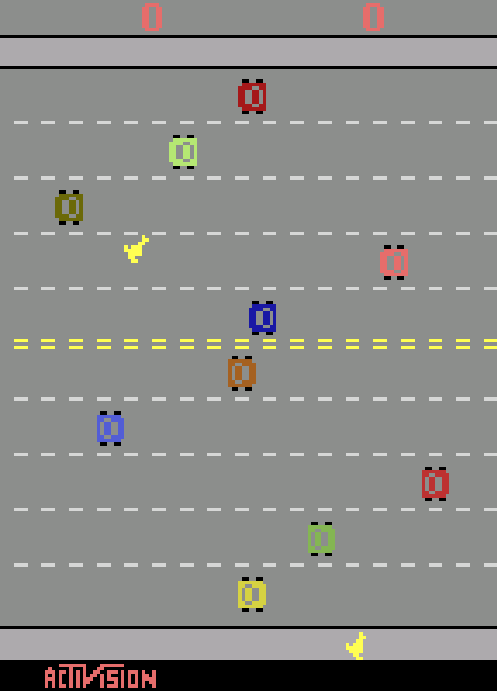
\includegraphics[width=0.5\textwidth,keepaspectratio]{figures/Freeway.png}
\caption[Sokoban]{Example of Freeway level}
\label{Fig.Boxing}
\end{figure}

\editnote{TODO: Add more games if needed.}

\subsubsection{Sokoban}

Sokoban is a classic planning problem. It is a challenging one-player puzzle game in which the goal is to navigate a grid world maze and push boxes onto target tiles. A Sokoban puzzle is considered solved when all boxes are positioned on top of target locations. The player can move in all 4 cardinal directions and only push boxes into an empty space (as opposed to pulling). For this reason many moves are irreversible and mistakes can render the puzzle unsolvable. A human player is thus forced to plan moves ahead of time. Artificial agents should similarly benefit from a learned model and simulation.

Despite its simple rule set, Sokoban is an incredibly complex game for which no general solver exists. It can be shown that Sokoban is NP-Hard and PSPACE-complete \cite{Benchmark.Sokoban}. Sokoban has an enormous state space that makes it inassailable to exhaustive search methods. An efficient automated solver for Sokoban must have strong heuristics, just as humans utilize their strong intuition, so that it is not overwhelmed by the number of possible game states.

The implementation of Sokoban\cite{Code.Sokoban} used for those experiments procedurally generates a new level each episode. This means an agent cannot memorize specific puzzles. Together with the planning aspect, this makes for a very challenging environment. While the underlying game logic operates in a 10 × 10 grid world, agents were trained directly on RGB sprite graphics. Fig.~\ref{Fig.Sokoban} shows an example of Sokoban level with 4 boxes and fig.~\ref{Fig.Sokoban_elements} explains the meaning of the visual icons.

\editnote{Note to the advisor: Do we need to go into deeper details about e.g. how rewards are obtained etc.? Or rather point to the repository for more information?}

\begin{figure}[H]
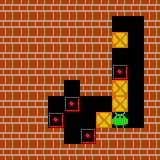
\includegraphics[]{figures/Sokoban.png}
\caption[Sokoban]{Example of Sokoban level (image size 160 × 160 pixels)}
\label{Fig.Sokoban}
\end{figure}

\subsection{Model learning}

First three experiments focus on training the world model in Sokoban environment. Because Sokoban is the deterministic environment, each experiment tested also the memory module without Mixture Density Network on top of a RNN. Instead a linear model was used to output the next latent state. \editnote{Note to the advisor: Should it be in the previous chapter (Planning with learned model a.k.a. project plan)?}

\subsubsection{Train the world model in the Sokoban environment}

In this experiment, the original world model was trained in the Sokoban environment. No modification to the original method described in the related work chapter was made, beyond addition of the deterministic variant of memory module.

The vision model successfully learned to encode high dimensional observations into low dimensional latent states. Fig.~\ref{Fig.Sokoban_vision} shows original observations (first and third columns) side by side with reconstructed observations from their encodings (second and fourth columns).

\begin{figure}[H]
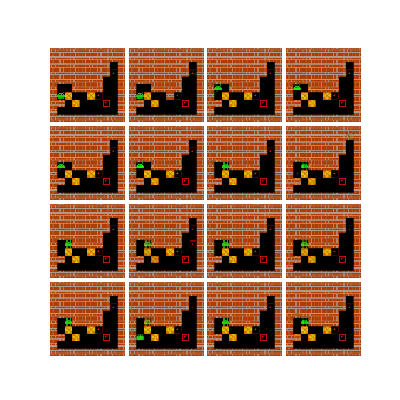
\includegraphics[width=1\textwidth,keepaspectratio]{figures/Sokoban_vision.png}
\caption[Qualitative result of the vision model training in Sokoban]{Qualitative result of the vision model training in Sokoban. First and third columns include original observations. Second and fourth columns include reconstructions. Each reconstruction was obtained by first encoding the original observation and then decoding, using VAE encoder and decoder respectively.}
\label{Fig.Sokoban_vision}
\end{figure}
\editnote{Make a better diagram.}

The stochastic and deterministic memory models were not able to learn Sokoban’s dynamics. Fig.~\ref{Fig.Sokoban_memory} shows that the stochastic model very often can not determine the agents position. The agent disappears and blocks change their types. The eighth row shows that pushing mechanics aren't modeled, the agent passes through boxes. The deterministic model don't do better.
The controller model failed to learn how to solve any level. We suspect that VAE is unable to generate usable abstract Sokoban representation and the shallow memory and controller models can not grasp complex dynamics of Sokoban using this poor representation.

\begin{figure}[H]
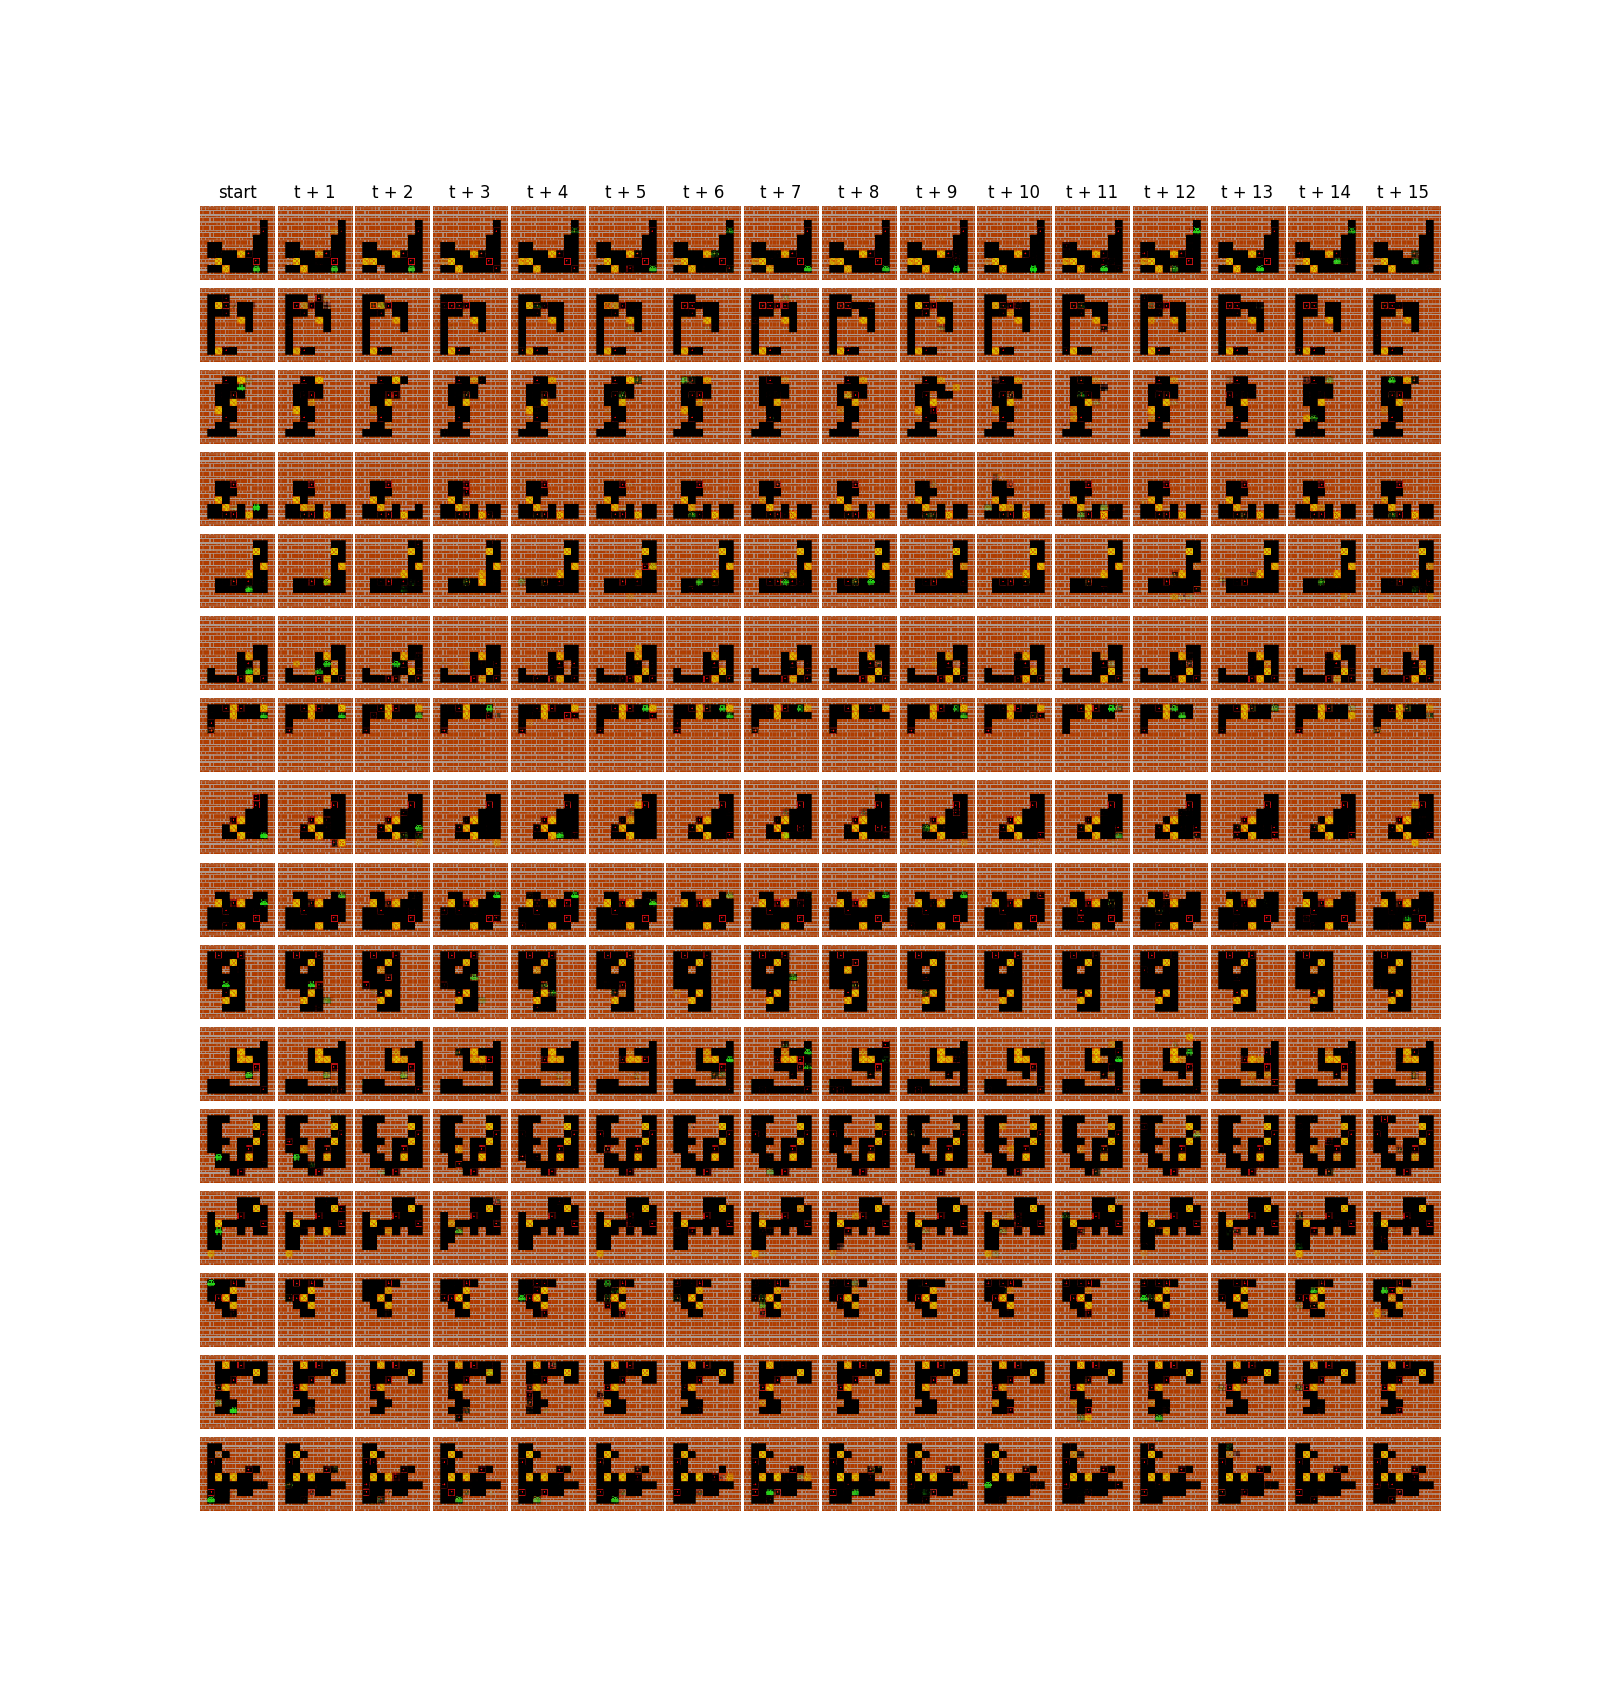
\includegraphics[width=1\textwidth,keepaspectratio]{figures/Sokoban_memory.png}
\caption[Qualitative result of the memory model training in Sokoban]{Qualitative result of the memory model training in Sokoban. Each row depicts the memory model rollout in one episode. The first column include original observations from the evaluation dataset from which the rollouts start. The RNN's hidden state was initialized on preceding transitions in each episode. Each subsequent reconstruction was obtained by first predicting the next latent state by the memory model and then decoding it using VAE decoder.}
\label{Fig.Sokoban_memory}
\end{figure}
\editnote{Make a better diagram.}
\editnote{Note to the advisor: Do we need to go into great detail about how it was generated? E.g. do we need to describe how the RNN was initialized or just point to the code?}

\subsubsection{Train the world model in Sokoban environment on 10x10 grid world states}

The latent state vector size is set to 64. This means that in theory this vector can accommodate full information about an observation. As noted before, Sokoban underlying game logic operates in a 10 × 10 grid world, where far edges of a level are always walls. This means that the level is described by 64 block types organized in an 8 x 8 grid. In this experiment, this domain knowledge is exploited and the agent uses those 64 block types as an input vector to the memory module, bypassing the vision model. It is worth noting, that the vision model should learn this representation as it is the optimal encoding when the objective is to compress a pixel image into a 64-dimensional vector and then reconstruct the original observation from it. However, despite use of the optimal encoding, the results have not been improved.

The proposed input format is optimal encoding if one wants to compress a pixel image and then reconstruct it. However, it is really poor representation of a current state of the environment if one wants to use linear combination of those features (block types in each position) to infer optimal next action and this is exactly what the controller model is tying to do. Modeling a value function could have more sense e.g. the value function could learn that a box on a target position yields higher value, but even it would have a hard time modeling more complex relations between entities in the environment. More useful for the controller would be e.g. representation that includes information about distance between the box and each target position. Nevertheless, this could be not enough too. The box on the target position would get discounted for not being on some other target positions. Hence, there is need for feature saying “the box X placed on the target position Y”. In the end, the linear combination of the proposed latent features can't model useful policy.

On the other hand, this representation includes, not well represented, but perfect information about an environment state. The memory model creates its own environment representation encoded in its hidden state and then uses this representation to predict the next latent state. This memory's hidden state is also utilized by the controller. Still, it doesn't seem to encode useful enough information for the two to do well on their tasks. One way to improve the hidden state representation is explored in the next experiment.

\subsubsection{Train the world model in Sokoban with auxiliary tasks}

Auxiliary tasks\cite{Algo.AuxiliaryTasks} have proved to help create more informative representation of an environment. In this experiment, reward and value prediction tasks are added to the memory model. In short, two additional linear models are added on top of the RNN to predict the next reward in the environment and model a value function. In theory, it should help form a more informative hidden state of the memory model. Consequently, it should help learn Sokoban’s dynamics, but also generate representation on a higher level of abstraction that could prove useful for the controller. Moreover, a reward prediction will be needed in further work on planning with learned model.

For all that, the memory model have not been able to learn to predict the rewards and values. Also, there was no improvement in memory's and controller’s performance. It is suspected, that the main cause of this failure are sparse rewards in the training dataset. A random agent used to generate the dataset does not receive many positive rewards. Effectively, most of the episodes do not have any positive reward. Hence, the memory model soon overfit on more or less constant reward and value. 
This yields insight that the data generation procedure does not cover state-space well. Iterative approach to gathering data, from a better and better agent, could solve this problem.

It is not without significance that Sokoban has enormous state-space. Each episode is much different from the others - it is nearly impossible for an agent to see a similar state in a different episode. Hence, Sokoban requires strong generalization capability from the memory module. Simple RNN can lack capacity to create good representation and in turn achieve good prediction performance. For instance I2A\cite{Algo.I2A} uses deep neural network architecture to handle Sokoban complexity. A more flexible memory model with larger capacity could manage this complexity and need for generalization. We explore those two insights in the next experiment with larger model and iterative training procedure.
 \newpage
\section{Conclusion}

The aim of this work is to propose model-based RL system, that could learn in complex high-dimensional environments. Deriving from state-of-the-art model learning \cite{Algo.RecurrentEnvSim}\cite{Algo.JointFrameRewardPrediction}\cite{Algo.FastGenerativeModels} and model-based RL \cite{Algo.SimPLe}\cite{Algo.VPN}\cite{Algo.WorldModels}\cite{Algo.PlaNet} techniques, three architectures are presented: ``Original World Models'' (OWM), ``World Models and AlphaZero'' (W+A) and ``Discrete PlaNet'' (DPN). Despite many difficulties, DPN finally reached a level of performance equal or higher than strong model-free and model-base baselines in low data regime of up to 1M interactions with the real environment of Atari 2600 game Boxing.

The most challenging part of this work, underestimated at first by the author, was model learning. Current state-of-the-art model learning methods, although report promising results, were not tested for planning with them using search based algorithms, let alone planning and learning. Towards the end of the experimentation phase for this thesis, the PlaNet paper came out. It become the keystone for the final solution: the DPN architecture.

Neither architecture was able to learn playing Sokoban. Certainly, the problem lies in model learning techniques. Sokoban dynamics, although based on simple rules of moving a character and pushing boxes, allow for incredible number of possible states and levels configurations. The models were not able to generalize well to this number of possibilities.

AlphaZero is very promising in a sense, that it is general reinforcement learning algorithm which proved to solve really complex problems, like playing the game of Go \cite{Algo.AlphaGoZero}, when supplied with the perfect environment dynamics model. It should easily manage Sokoban complexity. And yet, joining it with the imperfect learned world model resulted in unstable, and at the end unsuccessful, training. 

Likewise, for the DPN architecture, sparse rewards of Freeway became an obstacle which could not be overcome.

Future work could focus on extending this method to other challenging tasks like: sparse rewards environments, i.e. Freeway, and complex puzzle games with massive state-space sizes, i.e. Sokoban.
DPN, unlike model-based baseline SimPLe, hold promise of increased performance with an increased computational budget for planning. This hypothesis could be put to the extensive test too.
Furthermore, generalization of the DPN world model to different tasks in the same or very similar environments could be explored.
 \newpage

\renewcommand{\baselinestretch}{1.0}\normalsize	% żeby w wykazach była pojedyncza interlinia

\addcontentsline{toc}{section}{References}
\nocite{*}
\printbibliography
\newpage

\addcontentsline{toc}{section}{\listfigurename}
\listoffigures
\newpage

\addcontentsline{toc}{section}{\listtablename}
\listoftables

\renewcommand{\baselinestretch}{1.5}\normalsize	% powrót do interlinii 1.5 na wypadek dodatków

% nie dodawaj obrazków i tabel z dodatków do list powyżej
\let\svaddcontentsline\addcontentsline
\renewcommand\addcontentsline[3]{%
  \ifthenelse{\equal{#1}{lof}}{}%
  {\ifthenelse{\equal{#1}{lot}}{}{\svaddcontentsline{#1}{#2}{#3}}}}

\newpage

\begin{appendices}
\addtocontents{toc}{\protect\setcounter{tocdepth}{1}}

%\input{dodatki/gramatyka-opisu-klastra.tex} \newpage
%\input{dodatki/diagramy_komunikatow.tex} \newpage
\end{appendices}

\end{document}	% musi być na samiutkim końcu
